Esta sección busco que sea un diario de lo que voy aprendiendo a usar de este programa

\subsection{Convenciones}

El programa de CosmoLattice según el \href{https://arxiv.org/pdf/2102.01031}{manual} utiliza la siguiente lista de convenciones:

\begin{itemize}
    \item Unidades naturales $(c = 1, \ \hbar = 1)$.

    \item La signatura en la métrica es negativa para la parte temporal.

    \item Se usa la constante de gravitación $G$, la masa de Planck $M_p \simeq 1.22 \times 10^{19}$ GeV y la masa de Planck reducida $m_p \simeq 2.44 \times 10^{18}$ GeV, relacionadas a partir de $M_p^2 = 8 \pi m_p^2 = G^{-1}$.

    \item Los índices latinos son para las dimensiones espaciales, mientras que los griegos para las espacio-temporales. Pero salvo que se indique lo contrario, los índices repetidos no representan sumas.

    \item La métrica FLRW se considera como $ds^2 = - a^{2 \alpha} (\eta) \ d\eta^2 + a^2(\eta) \ \delta_{ij} \ dx^i \ dx^j$ con $\alpha$ un valor positivo y tal que $\alpha = 0$ es el tiempo coordenado y $\alpha = 1$ es el tiempo propio.

    \item La notación con punto para la derivada es para el tiempo cósmico mientras que la notación con apóstrofe es para derivadas respecto un tiempo de $\alpha$ arbitrario.

    \item El momento físico se representa con \textbf{p} mientras que el comovil se representa con \textbf{k}. A su vez, el parámetro de Hubble está dado por $\displaystyle \mathcal{H} = \frac{a^\prime}{a}$.

    \item Los parámetros cosmológicos son los que se obtienen del CMB en los experimentos de Planck.

    \item La convención de la transformada de Fourier es de la forma

    \begin{equation}
        f(\textbf{x}) = \frac{1}{(2\pi)^3} \int f(\textbf{k}) e^{ikx} \ d^3 k \hspace{2.5cm} f(\textbf{k}) = \int f(\textbf{x}) e^{-i k x} \ d^3 x
    \end{equation}

    \item La transformada de Fourier discreta (DFT) tiene por convención

    \begin{equation}
        f(\textbf{n}) =   \frac{1}{N^3} \sum_{\tilde{n}} \exp{\displaystyle i \frac{2 \pi}{N} \textbf{n} \textbf{$\tilde{n}$}} f(\textbf{$\tilde{n}$}) \hspace{2.5cm} f(\textbf{$\tilde{n}$}) =   \frac{1}{N^3} \sum_{n} \exp{- \displaystyle i \frac{2 \pi}{N} \textbf{n} \textbf{$\tilde{n}$}} f(\textbf{n})   
    \end{equation}
\end{itemize}

\subsection{Inicialización}

Por un lado, para la utilización armamos un \textit{conda environment} que llamaremos \textit{cosmolattice}, y que será creado a partir del archivo \textcolor{blue}{\href{https://drive.google.com/uc?export=download&id=1OmMo4wB7_Z4u8-0nX-I4SRWY4rsiE0yj}{\texttt{.yml}}} que me pasó Nahue con los paquetes necesarios para que corra correctamente.

Ahora, para usar CosmoLattice debemos comenzar clonando el repositorio del git como

\begin{lstlisting}[style = bashStyle]
git clone https://github.com/cosmolattice/cosmolattice.git
\end{lstlisting}

\noindent
dentro de este repositorio tendremos como carpetas las siguientes: \textit{dependencies} y \textit{src}, la primera tendrá los métodos que se usan para generar los cálculos, mientras que la segunda tiene los parámetros iniciales y los modelos físicos. Estos últimos están a su vez dentro de la carpeta \textit{models} y esta carpeta tiene por un lado los modelos que serán los ``.h'' y dentro de esta carpeta está la carpeta que dice \textit{parameter-files} que contiene los parámetros iniciales en los ``.in''.

\subsection{Comandos importantes}

\begin{infobox}[cyan]{Comentario}
    Dejo en mayúsculas MODELO y ARCHIVO para acordarme que ahí pongo lo que corresponda.
\end{infobox}

Primero hay que activar el entorno

\begin{lstlisting}[style = bashStyle]
conda activate cosmolattice
\end{lstlisting}

Creamos una carpeta dónde vamos a pedir que se generen los archivos

\begin{lstlisting}[style = bashStyle]
mkdir build_MODELO
\end{lstlisting}

Cargo el modelo a usar y crea el ejecutable al que hay que darle los parámetros iniciales

\begin{lstlisting}[style = bashStyle]
cmake -DMODEL=MODELO ../
make cosmolattice
\end{lstlisting}

Le doy condiciones iniciales al ejecutable y hago la simulación

\begin{lstlisting}[style = bashStyle]
./lphi4 input=../src/models/parameter-files/ARCHIVO.in
\end{lstlisting}

\subsection{04/07/2025}

Una vez hecho todo lo anterior empezamos a buscar entender cómo se arman los modelos y las condiciones iniciales a partir del modelo $\lambda \phi^4$ (archivos de nombre lphi4), entonces para entender un poco como funciona cada parte de estos archivos dejo asentado ésto

\subsubsection{Modelo}

Las líneas

\begin{lstlisting}[style = cppStyle]
#ifndef LPHI4_H
#define LPHI4_H
\end{lstlisting}

\noindent
se utilizan para evitar la inclusión múltiple del archivo. Si \texttt{LPHI4\_H} no está definido, se define; de lo contrario, se ignora el contenido para evitar que el archivo se incluya más de una vez, lo que podría causar errores. Esta protección se cierra con la instrucción \texttt{\#endif}.

Después, agregamos las dependencias con

\begin{lstlisting}[style = cppStyle]
#include "CosmoInterface/cosmointerface.h"
\end{lstlisting}

\noindent
que tiene las funciones básicas del código.

Las líneas

\begin{lstlisting}[style = cppStyle]
struct ModelPars : public TempLat::DefaultModelPars {
    static constexpr size_t NScalars = 2;
    static constexpr size_t NPotTerms = 2;
};
\end{lstlisting}

\noindent
marcan cuantos campos escalares tenemos (\texttt{NScalars}) y cuantos términos de potenciales tenemos (\texttt{NPotTerms}). Es importante recordar que los términos cinéticos los agrega por sí solos, sólo los potenciales debemos agregar nosotros.

Las líneas

\begin{lstlisting}[style = cppStyle]
#define MODELNAME lphi4

template<class R> 
using Model = MakeModel(R, ModelPars);
\end{lstlisting}

\noindent
permiten darle nombre al modelo con los parámetros definidos arriba.

Para definir las variables que nos van a ser de interés como los valores de las constantes de interacción usamos

\begin{lstlisting}[style = cppStyle]
private:
    double g, lambda, q;
\end{lstlisting}

\noindent
dónde las ponemos privadas para que sólo se usen dentro de este archivo. A su vez, vamos a usar

\begin{lstlisting}[style = cppStyle]
lambda = parser.get<double>("lambda");
q = parser.get<double>("q");
\end{lstlisting}

\noindent
en el modelo para decir que le doy el valor en un archivo externo.

El modelo va a ser creado a partir de

\begin{lstlisting}[style = cppStyle]
MODELNAME(ParameterParser& parser, RunParameters<double>& runPar, std::shared_ptr<MemoryToolBox> toolBox):
    Model<MODELNAME>(parser,runPar.getLatParams(), toolBox, runPar.dt, STRINGIFY(MODELLABEL))
{
    // inicializacion de parametros leyendo del archivo de entrada
    lambda = parser.get<double>("lambda");
    q = parser.get<double>("q");
    g = sqrt(q*lambda);

    // inicializacion de condiciones iniciales para campos y momentos
    fldS0 = parser.get<double, 2>("initial_amplitudes");
    piS0 = parser.get<double, 2>("initial_momenta", {0, 0});

    // parametros de reescalado
    alpha = 1;
    fStar = fldS0[0];
    omegaStar = sqrt(lambda) * fStar;

    setInitialPotentialAndMassesFromPotential();
}

\end{lstlisting}

\noindent
dónde \texttt{fStar}, \texttt{alpha} y \texttt{omegaStar} son parámetros para reescalar el tiempo y los campos a unidades internas del programa; por otro lado \texttt{fldSO} y \texttt{piSO} arreglos con las condiciones iniciales de los campos y sus momentos.

Los términos potenciales los definimos a partir de

\begin{lstlisting}[style = cppStyle]
auto potentialTerms(Tag<0>) {
    return 0.25 * pow<4>(fldS(0_c));
}

auto potentialTerms(Tag<1>) {
    return 0.5 * q * pow<2>(fldS(0_c) * fldS(1_c));
}

\end{lstlisting}

\noindent
en este caso los términos potenciales son $\displaystyle \frac{1}{4} \phi^4$ y $\displaystyle \frac{g}{2} \phi^2 \chi^2$. A su vez, también debemos definir las derivadas primera y segunda de este potencial porque no las puede calcular solas y eso lo hacemos con

\begin{lstlisting}[style = cppStyle]
auto potDeriv(Tag<0>) {
    return pow<3>(fldS(0_c)) + q * fldS(0_c) * pow<2>(fldS(1_c));
}

auto potDeriv(Tag<1>) {
    return q * fldS(1_c) * pow<2>(fldS(0_c));
}

auto potDeriv2(Tag<0>) {
    return 3 * pow<2>(fldS(0_c)) + q * pow<2>(fldS(1_c));
}

auto potDeriv2(Tag<1>) {
    return q * pow<2>(fldS(0_c));
}
\end{lstlisting}

\subsubsection{Condiciones iniciales}

La línea

\begin{lstlisting}[style = cppStyle]
outputfile = ./
\end{lstlisting}

\noindent
sirven para definir el lugar dónde se guardarán los datos, en este caso es el directorio actual.

Las líneas

\begin{lstlisting}[style = cppStyle]
expansion = true
evolver = VV2
\end{lstlisting}

\noindent
sirven para prender la evolución temporal y \texttt{VV2} es el tipo de integrador que usará para calcular el factor de escala.

Los parámetros no independientes entre sí que nos darán de cierto modo la resolución del Lattice son

\begin{lstlisting}[style = cppStyle]
N = 32
dt = 0.05
kIR = 0.2
\end{lstlisting}

\noindent
dónde \texttt{N} son las divisiones en la caja, al ponerle 32 le estamos diciendo que cada dimensión la separe en 32 divisiones, \texttt{dt} es el paso de integración y \texttt{kIR} es el valor de corte para el número de onda infrarroja, o sea el mínimo $k$ al que podrá trabajar.

Cada cuanto guardo los datos estará dado por

\begin{lstlisting}[style = cppStyle]
tOutputFreq = 0.1
tOutputInfreq = 1
tMax = 300
\end{lstlisting}

\noindent
dónde \texttt{tOutputFreq} es la frecuencia en que guardo tiempos de cosas ligeras (campos, energías, entre otros), \texttt{tOutputInfreq} es el intervalo de tiempo en que guardo cosas más pesadas (tensores, espectros, entre otros), y \texttt{tMax} es el tiempo máximo al que llegará la simulación.

Cosas que no vamos a cambiar son

\begin{lstlisting}[style = cppStyle]
PS_type = 1
PS_version = 1
\end{lstlisting}

\noindent
que es la forma en la que calcula el espectro de potencias.

Para prender que dé un espectro de salidas de ondas gravitatorias tenemos

\begin{lstlisting}
GWprojectorType = 1
withGWs = true
\end{lstlisting}

\noindent
dónde \texttt{true} prende esta salida y el \texttt{GWprojectorType} es la forma en la que aplica el proyector TT para obtener la parte tensorial de las perturbaciones.

Para setear las condiciones iniciales tenemos

\begin{lstlisting}[style = cppStyle]
kCutOff = 4
initial_amplitudes = 5.6964e18 0   # en GeV
initial_momenta = -4.86735e30 0    # en GeV^2
\end{lstlisting}

\noindent
dónde \texttt{kCutOff} es el valor máximo de $k$ y la otra parte permite crear un arreglo de amplitudes iniciales y momentos iniciales.

Finalmente, el código define valores para $\lambda$ y $q$ a partir de

\begin{lstlisting}[style = cppStyle]
lambda = 9e-14
q = 0
\end{lstlisting}

\subsubsection{Levantar los espectros}

El CosmoLattice deja archivos con todas las cuentas hechas para entender la evolución en recalentamiento pero para visualizarlos debemos usar Python.

Hoy usamos el código que me pasó Nahue, pero falta sentarse a entenderlo línea por línea.

Para empezar, las librerías que usaremos y los parámetros para los gráficos los tendremos en las siguientes líneas:

\begin{lstlisting}[style = pythonStyle]
import numpy as np
import matplotlib as mpl
import matplotlib.pyplot as plt

%matplotlib inline       

mpl.rc('text', usetex = True)
mpl.rc('font', family = 'serif')
mpl.rc('font', size = '14')
mpl.rc('xtick', labelsize=14) 
mpl.rc('ytick', labelsize=14) 

dir = "./"
\end{lstlisting}

El archivo \texttt{average\_scale\_factor.txt} que formamos con CosmoLattice tienen las siguientes columnas: 

\begin{center}
    \begin{tabular}{|c|c|c|c|}
        $\eta$ & $a$ & $a^\prime$ & $\displaystyle \frac{a^\prime}{a}$  \\
    \end{tabular}
\end{center}

\noindent
para leer este archivo y poder usarlo después usamos

\begin{lstlisting}[style = pythonStyle]
expansion = True

if expansion == True:
    # load the file in aDat
    aDat = np.loadtxt(dir + "average_scale_factor.txt")
    
    #plot a
    plt.figure(0)
    plt.plot(aDat[:,0], aDat[:,1])
    plt.ylabel("$a$")
    plt.xlabel('$\\tilde\eta$')
    
    #plot a'
    plt.figure(1)
    plt.plot(aDat[:,0], aDat[:,2])
    plt.ylabel("$a'$")
    plt.xlabel('$\\tilde\eta$')
    
    
    #plot a'/a
    plt.figure(2)
    plt.plot(aDat[:,0], aDat[:,3])
    plt.ylabel("$a'/a$")
    plt.xlabel("$\\tilde\eta$");

else:
    aDat = None
\end{lstlisting}

El resto de los archivos de promedios sobre los campos tienen en sus columnas la siguiente información:

\begin{center}
    \begin{tabular}{|c|c|c|c|c|c|c|}
        $\eta$ & $\langle \tilde\phi_n \rangle$ & $\langle \tilde\phi'_n \rangle$ & $\langle \tilde\phi^2_n \rangle$ & $\langle \tilde\phi^{'2}_n \rangle$ & $\mathrm{rms}(\tilde\phi_n) $ & $\mathrm{rms}(\tilde\phi'_n) $
    \end{tabular}
\end{center}

\noindent
para graficar estos archivos, se define la función de graficar como

\begin{lstlisting}[style = pythonStyle]
def plot_fld(fldDat, fldNum="", aDat=None):
    plt.figure(0)
    plt.plot(fldDat[:,0], fldDat[:,1])
    plt.xlabel("$\\tilde\eta$")
    plt.ylabel("$\langle\phi_"+ fldNum +"\\rangle$")
    
    if aDat is not None:
        plt.figure(1)
        plt.plot(fldDat[:,0], aDat[:,1] * fldDat[:,1])
        plt.xlabel("$\\tilde\eta$")
        plt.ylabel("$a\cdot\langle\phi_"+ fldNum +" \\rangle$")
    
        plt.figure(2)
        plt.plot(fldDat[:,0], aDat[:,1] * fldDat[:,5])
        plt.xlabel("$\\tilde\eta$")
        plt.ylabel("$a\cdot\mathrm{rms}(\phi_"+ fldNum +")$")
        plt.yscale('log')
\end{lstlisting}

Para ver la conservación de energía, los archivos están compuestos por

\begin{center}
    \begin{tabular}{|c|c|c|c|}
        $\tilde\eta$ & $\frac{\langle LHS - RHS\rangle}{\langle LHS + RHS\rangle}$ & $\langle LHS \rangle$ & $\langle RHS \rangle$
    \end{tabular}
\end{center}

Para la densidad de energía, los archivos son de la forma

\begin{center}
    \begin{tabular}{|c|c|c|c|c|c|c|c|c|c|}
        $\tilde\eta$ & $\tilde E_K^{(0)}$ & $\tilde E_G^{(0)}$ & $\dots$ & $\tilde E_K^{(N_s-1)}$ & $\tilde E_G^{(N_s-1)}$ &  $\tilde E_V^{(0)}$ & $\dots$ &  $\tilde E_V^{(N_p-1)}$ & $\langle \tilde \rho \rangle$
    \end{tabular}
\end{center}

\noindent
para este último archivo, podemos graficar según si tenemos expansión del universo o no de la siguiente forma

\begin{lstlisting}[style = pythonStyle]
enDat = np.loadtxt(dir + "average_energies.txt")

nColumns = np.shape(enDat)[1]

# set explicitly different colors, so we know who is who
colors = ["tab:blue", "tab:orange", "tab:green", 
          "tab:red", "tab:purple", "tab:brown", "tab:pink"]

if expansion == True:
    plt.figure(0)
    for i in range(1,nColumns):
        plt.plot(enDat[:,0], aDat[:,1]**4 * enDat[:,i], color = colors[i-1])
        plt.yscale('log')
        plt.xlabel("$\\tilde \eta$")
        plt.ylabel("$\langle \\rho's\\rangle$")
        
    plt.figure(1)
    for i in range(1,nColumns):
        plt.plot(enDat[:,0], aDat[:,1]**4 * enDat[:,i], color = colors[i-1])
        plt.xlabel("$\\tilde \eta$")
        plt.ylabel("$\langle \\rho's\\rangle$")
else:
    plt.figure(0)
    for i in range(1,nColumns):
        plt.plot(enDat[:,0], enDat[:,i], color = colors[i-1])
        plt.yscale('log')
        plt.xlabel("$\\tilde \eta$")
        plt.ylabel("$\langle \\rho's\\rangle$")
        
    plt.figure(1)
    for i in range(1,nColumns):
        plt.plot(enDat[:,0], enDat[:,i], color = colors[i-1])
        plt.xlabel("$\\tilde \eta$")
        plt.ylabel("$\langle \\rho's\\rangle$")
\end{lstlisting}

Los archivos de los espectros se forman así:

\begin{center}
    \begin{tabular}{|c|c|c|c|c|}
        $\tilde k$ & $\tilde\Delta_{\tilde\phi}$ & $\tilde\Delta_{\tilde\phi'}$ & $\tilde n_{\tilde\phi}$ & bin multiplicity
    \end{tabular}
\end{center}

\noindent
el archivo también define a las funciones que leen y grafican al espectro como

\begin{lstlisting}[style = pythonStyle]
def load_spectrum(filename, comment = '#'):
    # The next few lines open the file and count
    # how many bins in one spectrum
    file = open(filename)
    nBins = 0
    # read first line
    line = file.readline()
    # while no blank we continue
    while line != "\n":
        # if not a comment line (header for instance)
        # we count one line
        if(line[0] != comment):
            nBins +=1
        # read next line
        line = file.readline()
    file.close()

    # now we know nBins. We still need to actually read the data.
    fileSp = np.loadtxt(filename, comments=comment)

    # find how many spectra are in the files
    nSpectra = len(fileSp) / nBins

    return fileSp, int(nBins), int(nSpectra)


def plot_spectrum(spectra, column, nBins, nSpectra, colormap = 'plasma'):
    colors = plt.get_cmap(colormap)
    for i in range(nSpectra):
        plt.plot(spectra[i*nBins:(i+1)*nBins,0], spectra[i*nBins:(i+1)*nBins,column], color=colors(i/nSpectra))
    plt.xscale('log')
    plt.yscale('log')
    plt.xlabel('$\\tilde k$')
\end{lstlisting}

\subsection{$\lambda \phi^4$ sin expansión}

Para empezar a entender cómo funciona CosmoLattice vamos a aprender cómo varía el espectro de potencias para el inflatón y para el campo hijo como a su vez cómo cambia el espectro de ondas gravitacionales.

Hay que tener en cuenta a la hora de cambiar parámetros que nos va a interesar cómo cambian estos espectro con el tiempo, con $N$ (el número de puntos), $k_{IR}$ (el valor más bajo de $k$ que pueda calcular), $k_{cutoff}$ (el valor más alto de modos con condiciones iniciales no nulas) y el tiempo de simulación. Además, el determinar $N$ y $k_{IR}$ fuerza a que el máximo valor de $k$ que pueda calcular va a estar dado por 

\begin{equation}
    k_{max} = \frac{\sqrt{3}}{2} N k_{IR}
\end{equation}

\noindent
y cuando corramos una simulación tenemos que tener en cuenta que el incremento en pasos temporales y espaciales deben cumplir la relación de estabilidad de Courant para que sea fiable, esta relación nos indica

\begin{equation}
    \frac{\delta \eta}{\delta x} < \frac{1}{\sqrt{N_{dims}}}
\end{equation}

\noindent
$\delta \eta$ se puede encontrar en el código .in, pero $\delta x$ lo podemos encontrar usando $k_{IR}$ a partir de 

\begin{equation}
    \delta x = \frac{2 \pi}{N k_{IR}}
\end{equation}

A partir de todas las consideraciones anteriores, vamos a querer empezar a caracterizar los espectros para algún $q$ fijo y ver cómo cambian respecto a $N$, en el sentido de querer comparar con los códigos armados de $\lambda \phi^4$ en el régimen lineal, entonces vamos a utilizar $q = 5050$ y $k_{cutoff} = 100$ y buscar cómo cambia la posición de los picos del espectro cuando cambio $N$ en $64$, $128$ y $256$, hay que tener en cuenta que $k_{IR}$ hay que dejarlo fijo para mantener la mayor fidelidad por tanto para poder comparar tomamos $k_{IR} = 0.02$ y obtenemos los espectros que se observan en la figura \ref{fig:cosmolattice_varN}. En los espectros obtenidos podemos notar que aumenta el $k_{max}$ obtenido, además aumenta la resolución con el aumento de $N$ junto a eso se puede ver que para valores grandes de $k$ se forma una panza independiente del $N$ lo que nos indica que al final de los valores de $k$ siempre tendremos ésto; al igual que ocurre para modos chicos que hay otra panza independiente del $N$.

\begin{figure}[H]
    \centering
    \begin{subfigure}[t]{\linewidth}
        \centering
        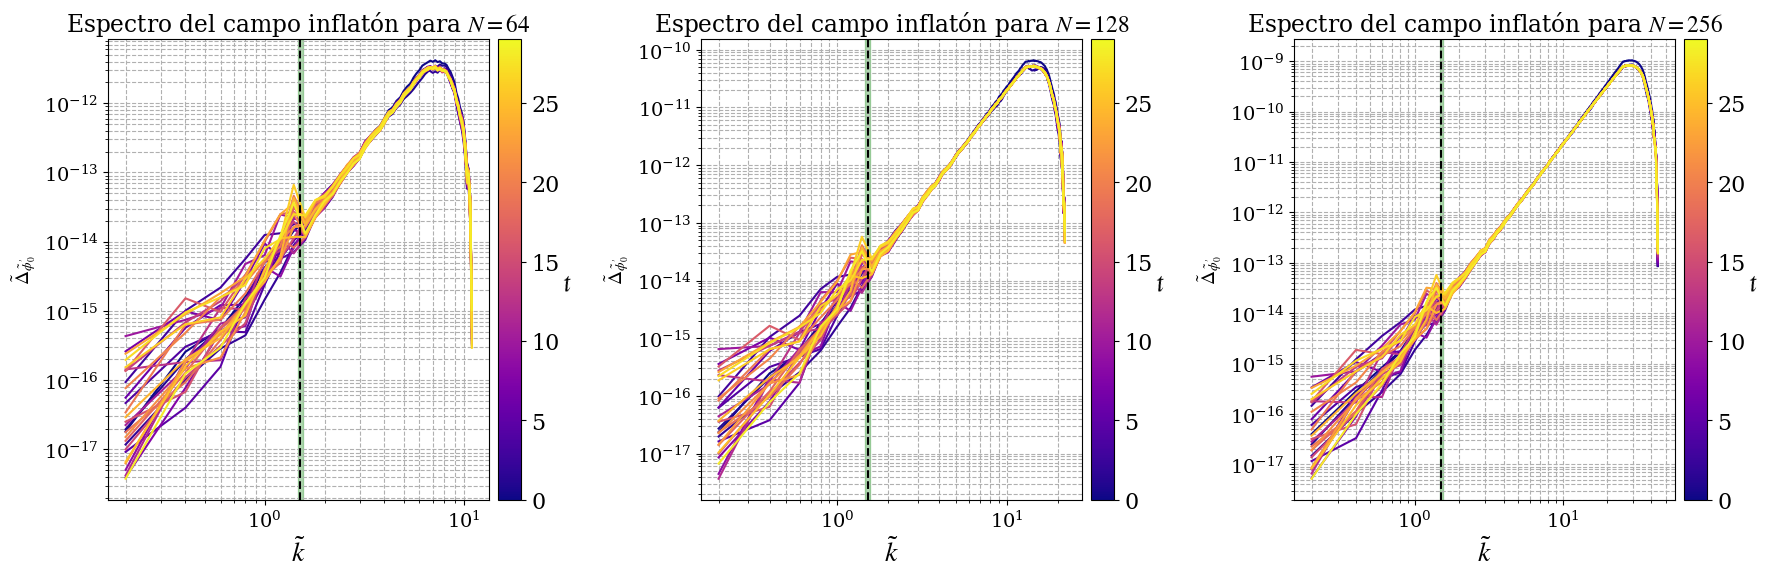
\includegraphics[width = \linewidth]{Imagenes/cosmolattice/varN_inflaton.png}
        \caption{espectro de potencias del inflatón}
    \end{subfigure}
    \begin{subfigure}[t]{\linewidth}
        \centering
        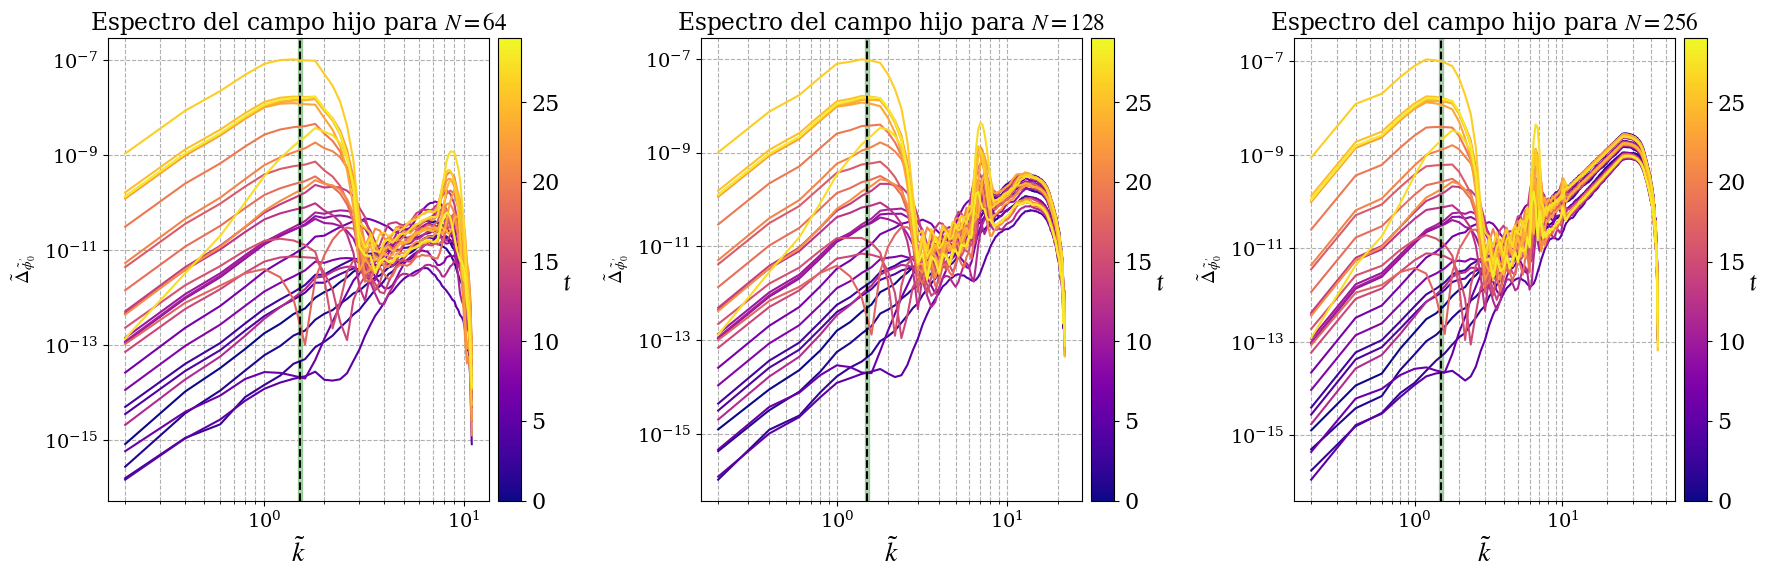
\includegraphics[width = \linewidth]{Imagenes/cosmolattice/varN_hijo.png}
        \caption{espectro de potencias del campo hijo}
    \end{subfigure}
    \begin{subfigure}[b]{\linewidth}
        \centering
        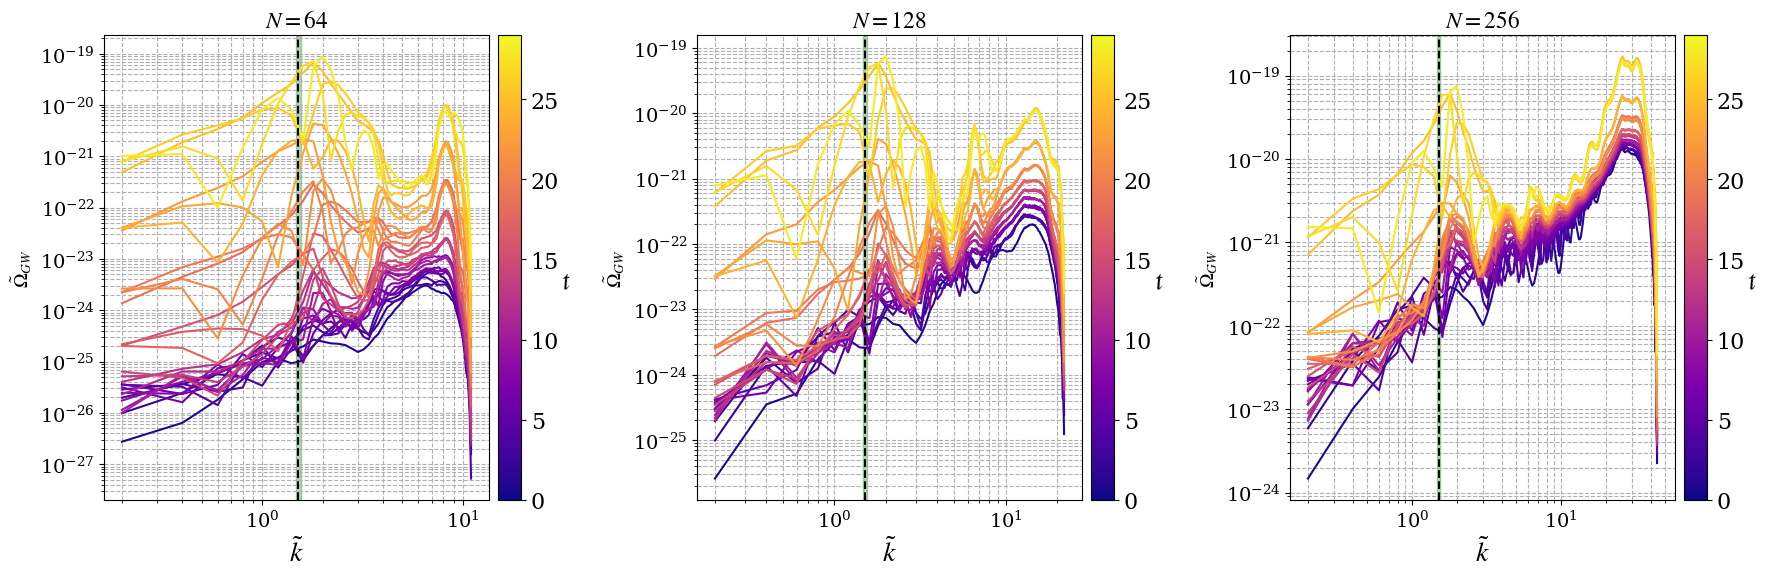
\includegraphics[width = \linewidth]{Imagenes/cosmolattice/varN_GW.png}
        \caption{espectro de potencias de las ondas gravitacionales}
    \end{subfigure}
    \caption{espectros obtenidos al variar $N$}
    \label{fig:cosmolattice_varN}
\end{figure}

Ahora, hagamos el mismo análisis dejando $N = 256$ para tener la máxima resolución en $k$'s pero variemos $k_{IR}$ para ver cómo depende el programa con este parámetro, ésto lo podemos ver en la figura \ref{fig:cosmolattice_varkIR}. Podemos nuevamente encontrar los mismos objetos extraños que antes, hay dos panzas que parecería pensar que para tiempos cortos no resuelve bien el código: una para $k$ chicos y otra para $k$ grandes. A su vez podemos ver que el pico a menos de algunos corrimientos se encuentra en la zona de amplificación que calculamos con Floquet.


\begin{figure}[H]
    \centering
    \begin{subfigure}[t]{\linewidth}
        \centering
        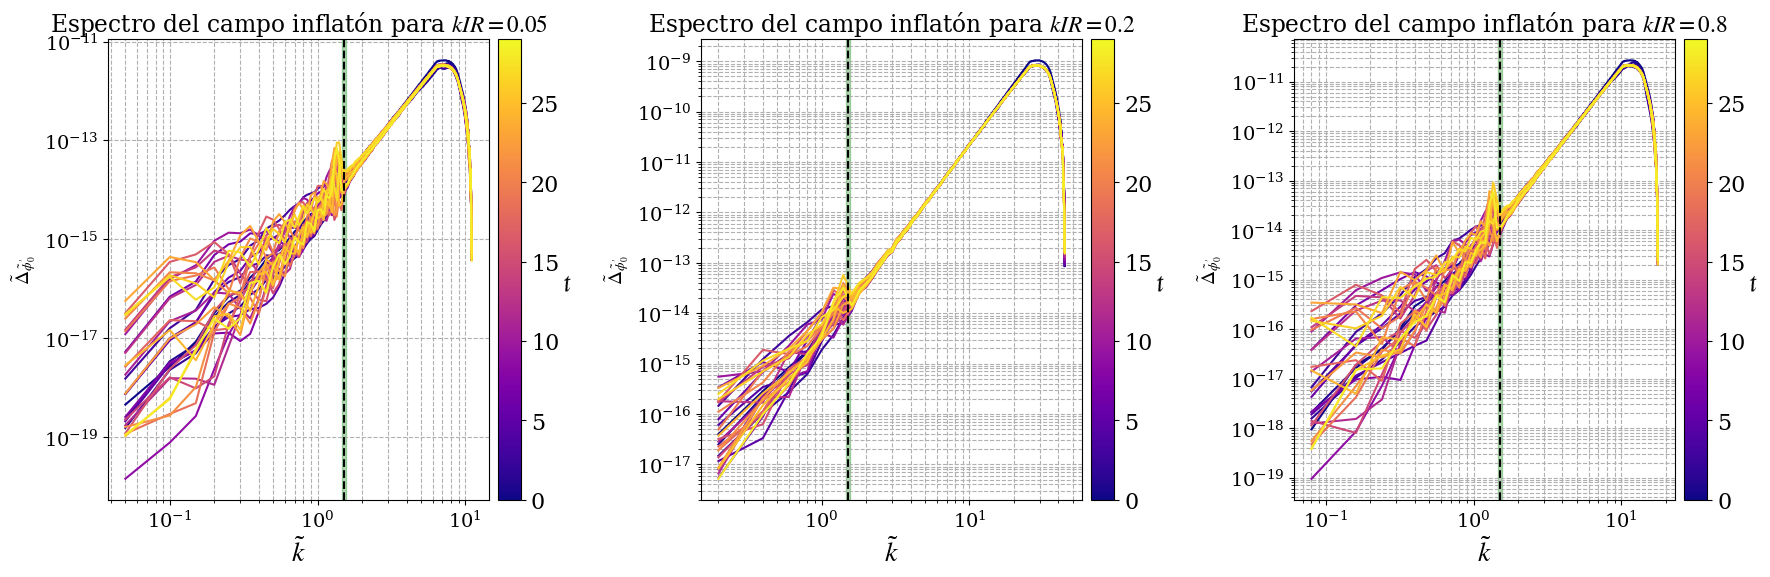
\includegraphics[width = \linewidth]{Imagenes/cosmolattice/varkIR_inflaton.png}
        \caption{espectro de potencias del inflatón}
    \end{subfigure}
    \begin{subfigure}[t]{\linewidth}
        \centering
        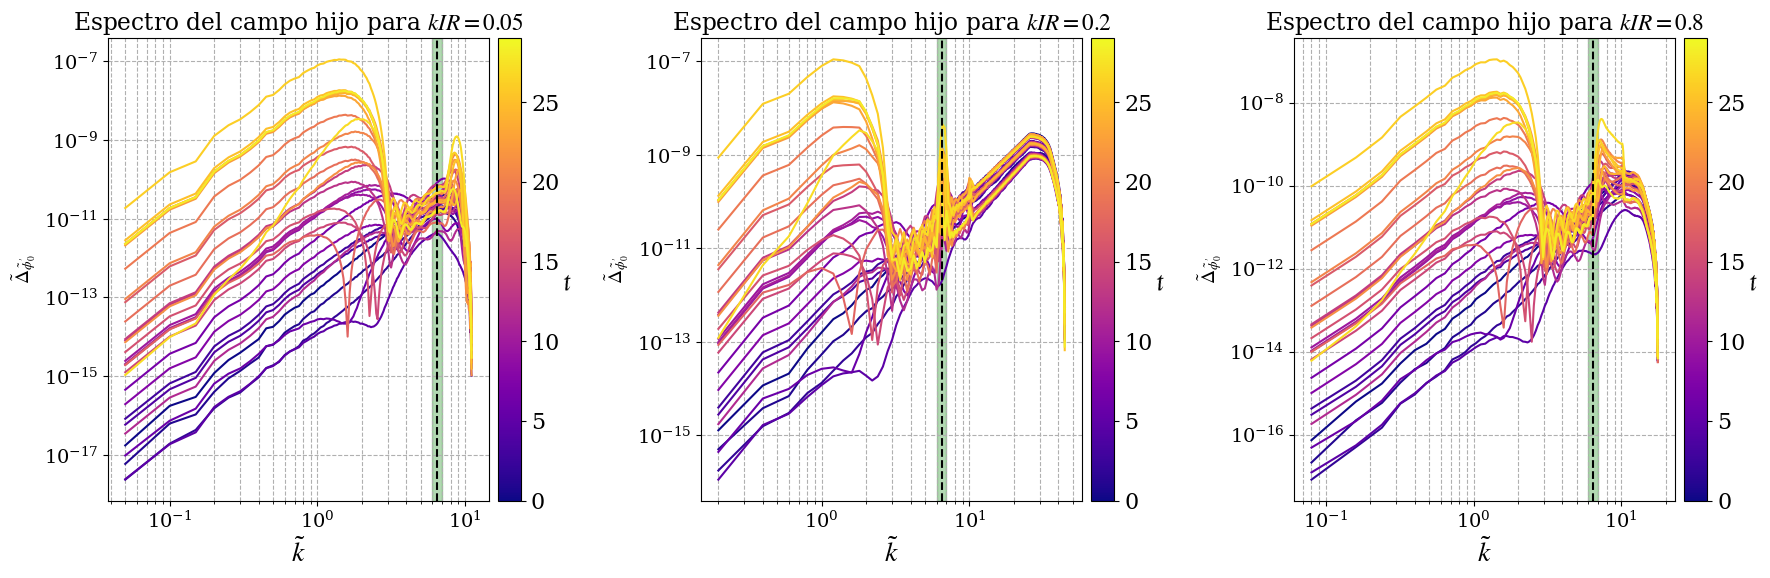
\includegraphics[width = \linewidth]{Imagenes/cosmolattice/varkIR_hijo.png}
        \caption{espectro de potencias del campo hijo}
    \end{subfigure}
    \begin{subfigure}[b]{\linewidth}
        \centering
        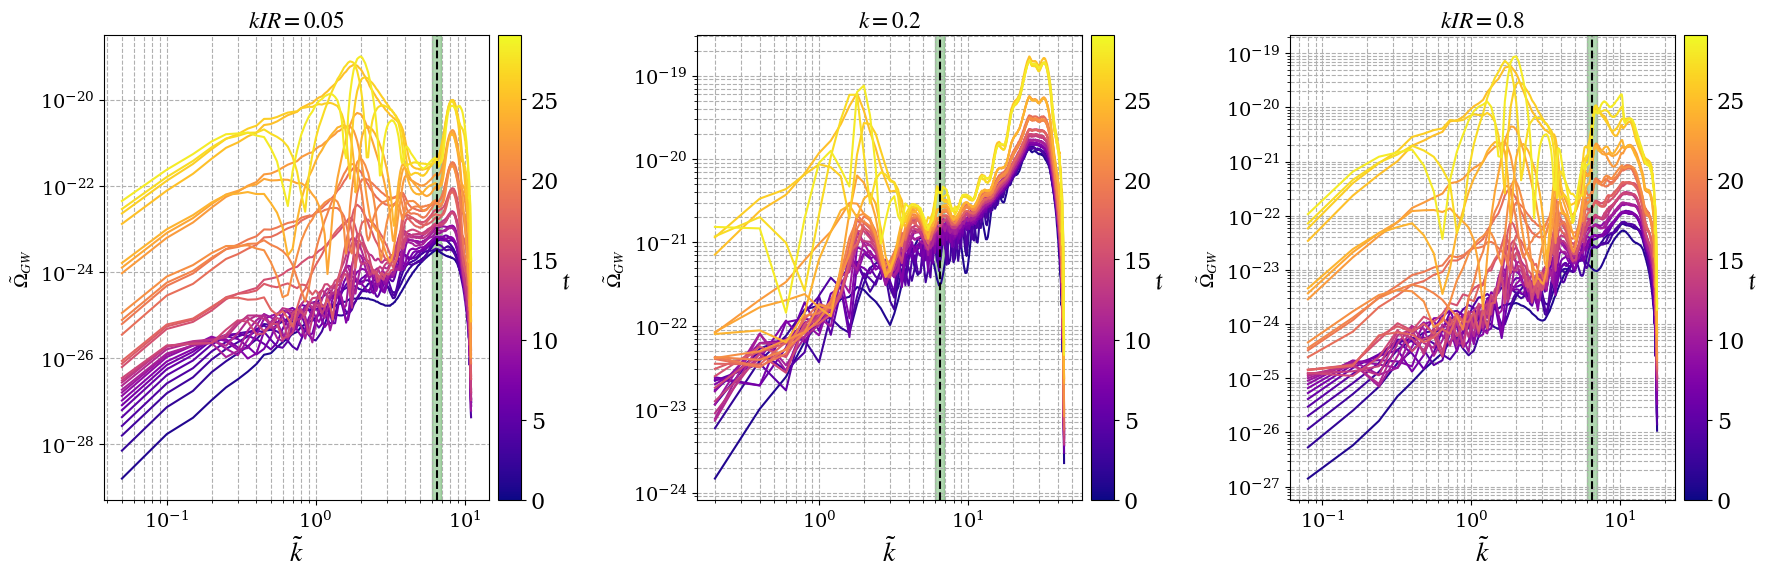
\includegraphics[width = \linewidth]{Imagenes/cosmolattice/varkIR_GW.png}
        \caption{espectro de potencias de las ondas gravitacionales}
    \end{subfigure}
    \caption{espectros obtenidos al variar $kIR$}
    \label{fig:cosmolattice_varkIR}
\end{figure}

Finalmente, lo último que podemos variar para ver cómo cambia la idea de comparar el pico de ondas gravitacionales y los espectros de potencia en función con el análisis de Floquet, para eso variamos $q$ dejando $k_{IR} = 0.2$, $k_{cutoff} = 100$ y $N = 256$ fijos. Estas comparaciones las podemos ver en la figuras \ref{fig:cosmolattice_varq_inf}, \ref{fig:cosmolattice_varq_chi} y \ref{fig:cosmolattice_varq_GW} dónde podemos notar que las figuras del inflatón son similares lo que nos indica que está bien, el espectro del campo hijo podemos encontrarnos nuevamente con las panzas al igual que con GW y eso genera que para algunos $q$'s no podamos identificar los picos en los espectros no pudiendo comparar con el modelo de Floquet propuesto.

\begin{figure}[H]
    \centering
    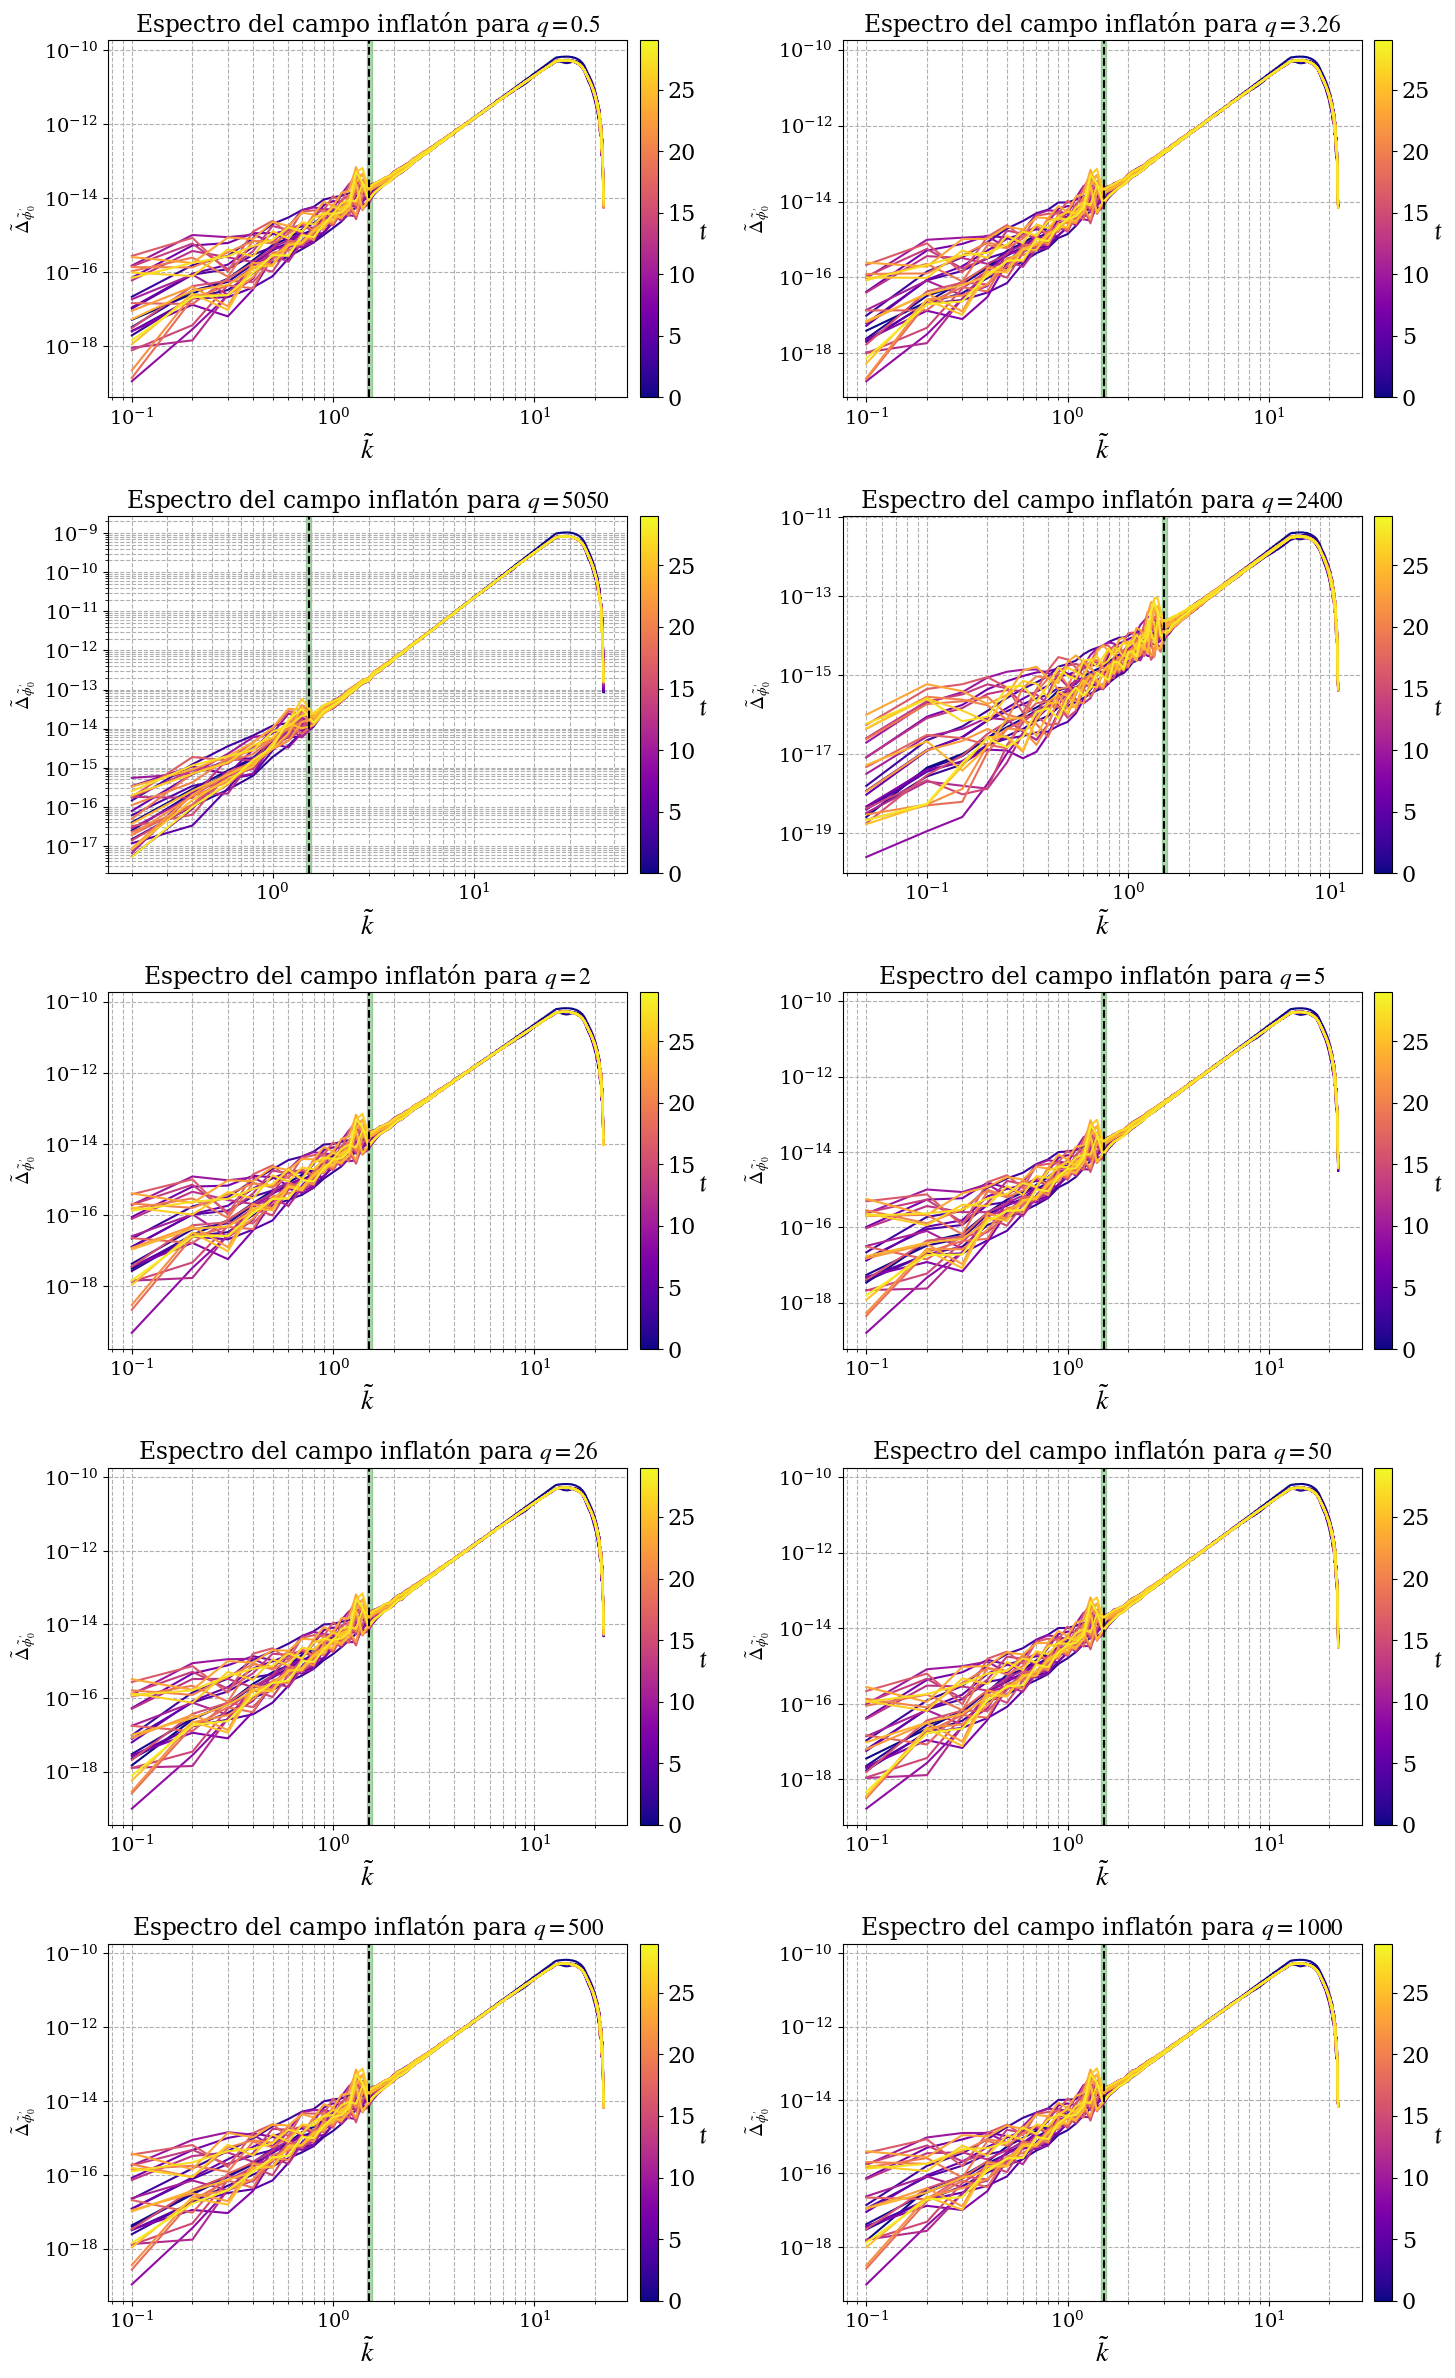
\includegraphics[width = \linewidth]{Imagenes/cosmolattice/varq_inflaton.png}
    \caption{espectro del inflatón para distintos $q$.}
    \label{fig:cosmolattice_varq_inf}
\end{figure}

\begin{figure}[H]
    \centering
    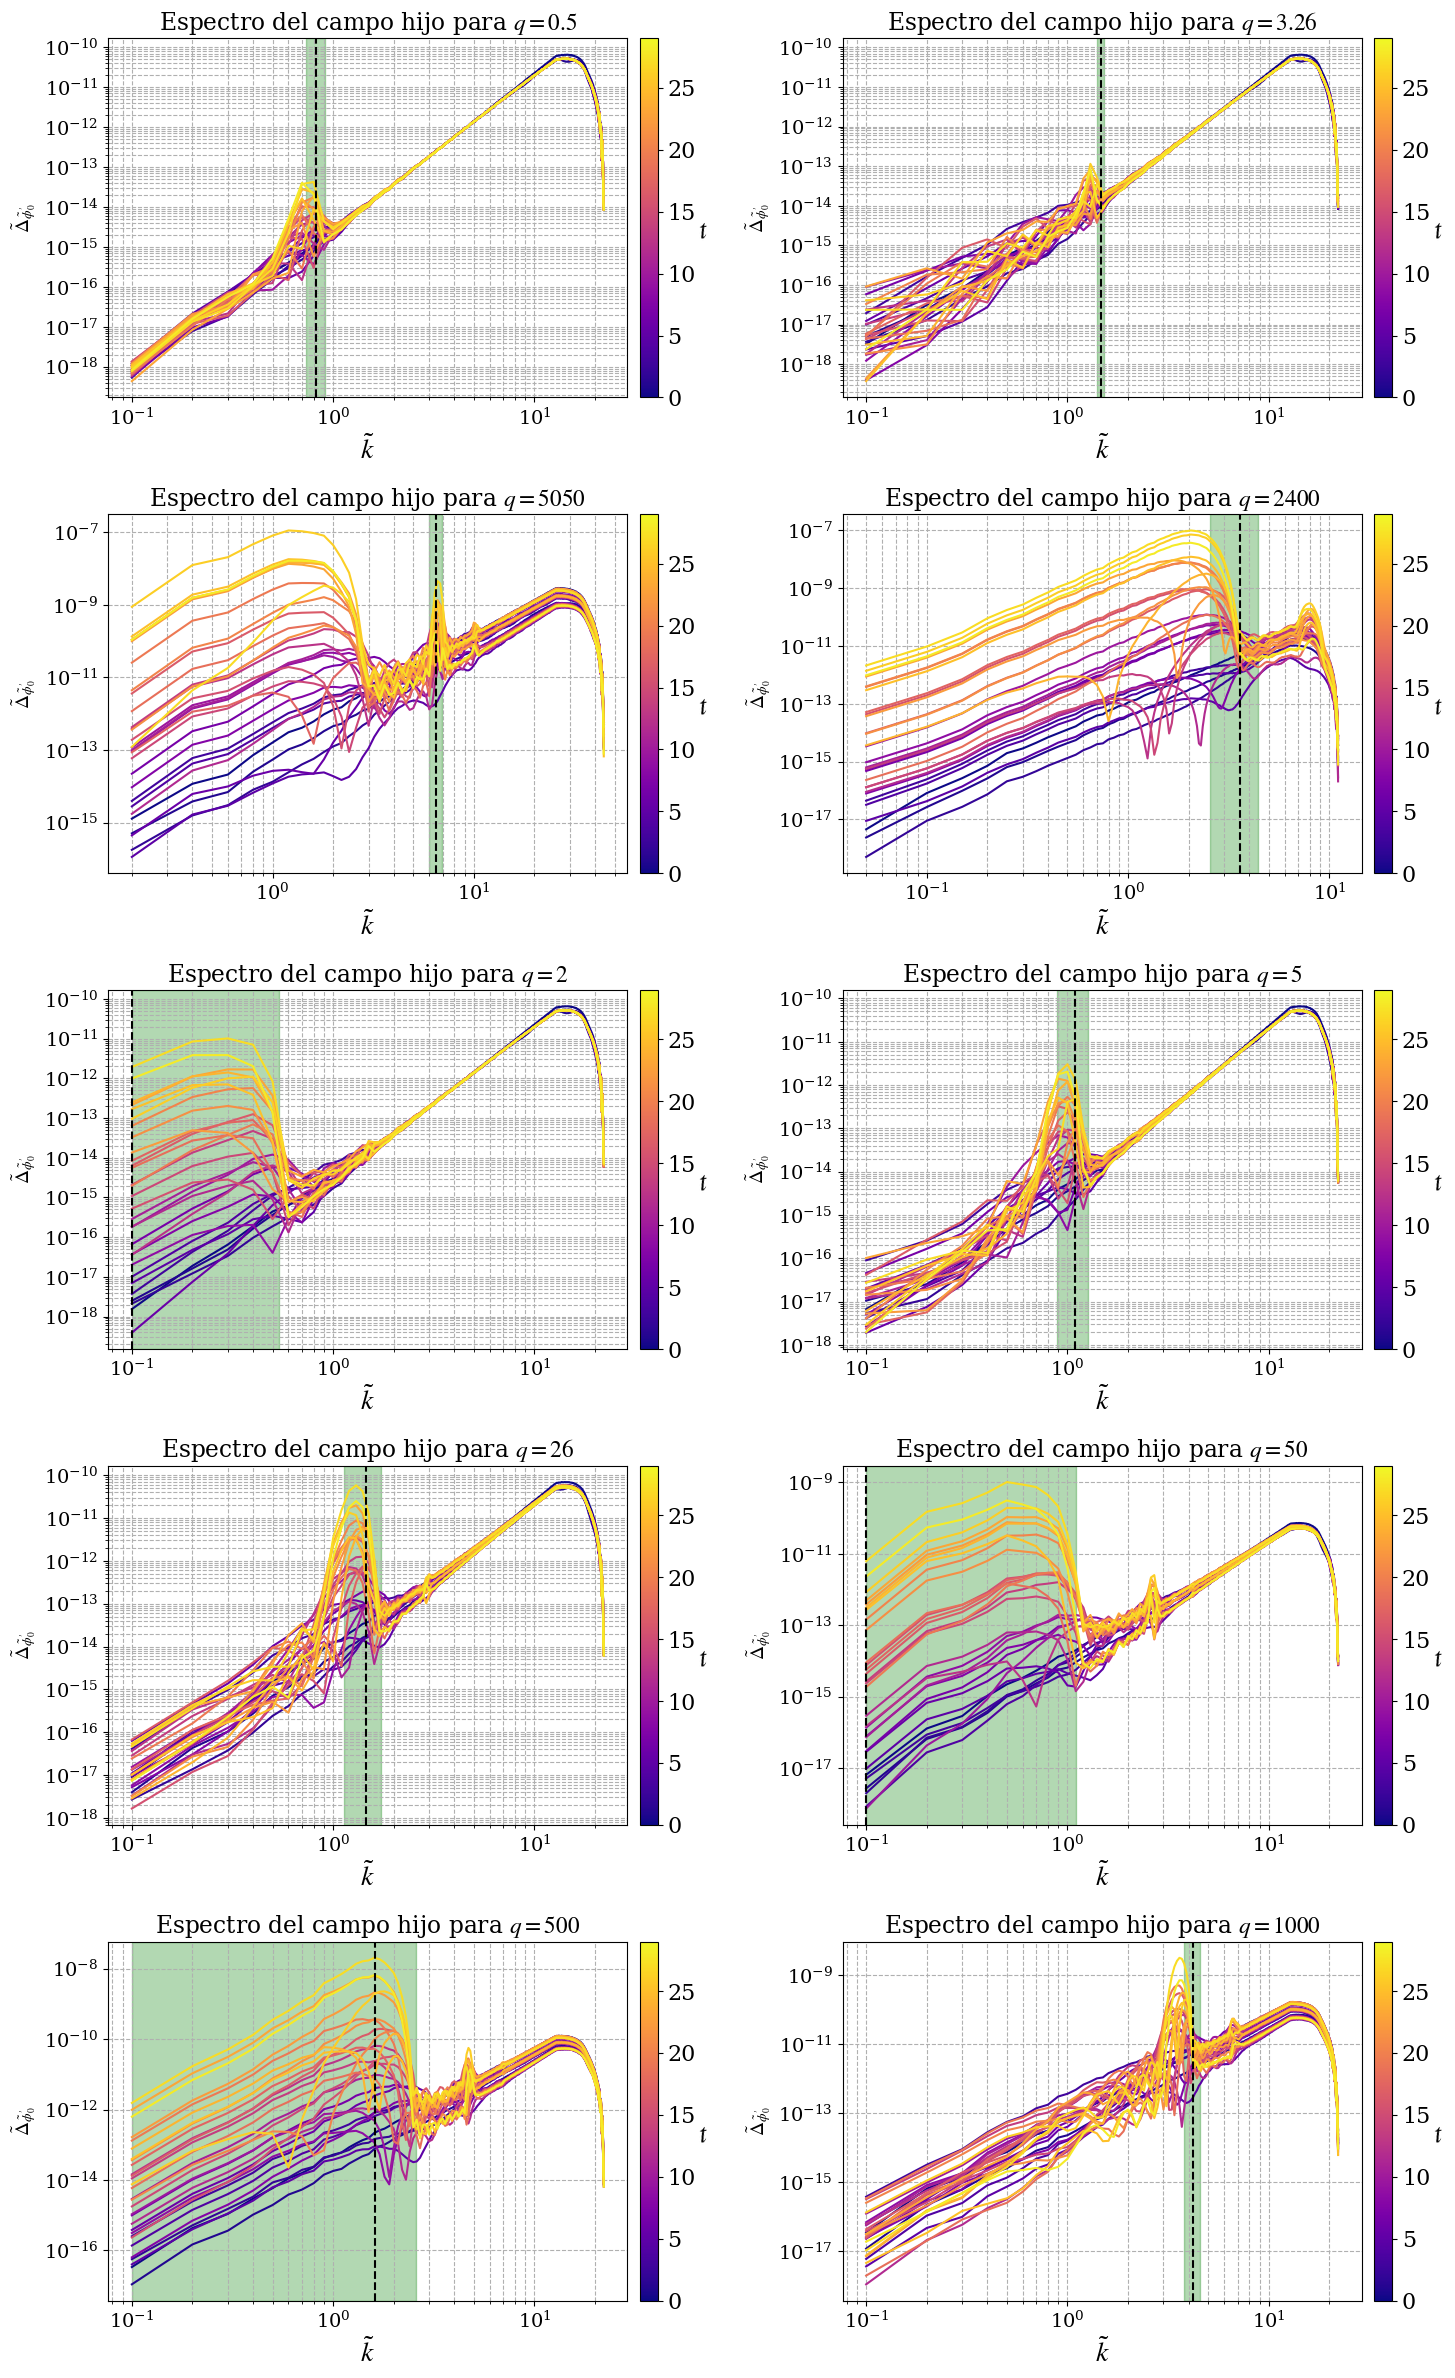
\includegraphics[width = \linewidth]{Imagenes/cosmolattice/varq_hijo.png}
    \caption{espectro del campo hijo para distintos $q$.}
    \label{fig:cosmolattice_varq_chi}
\end{figure}

\begin{figure}[H]
    \centering
    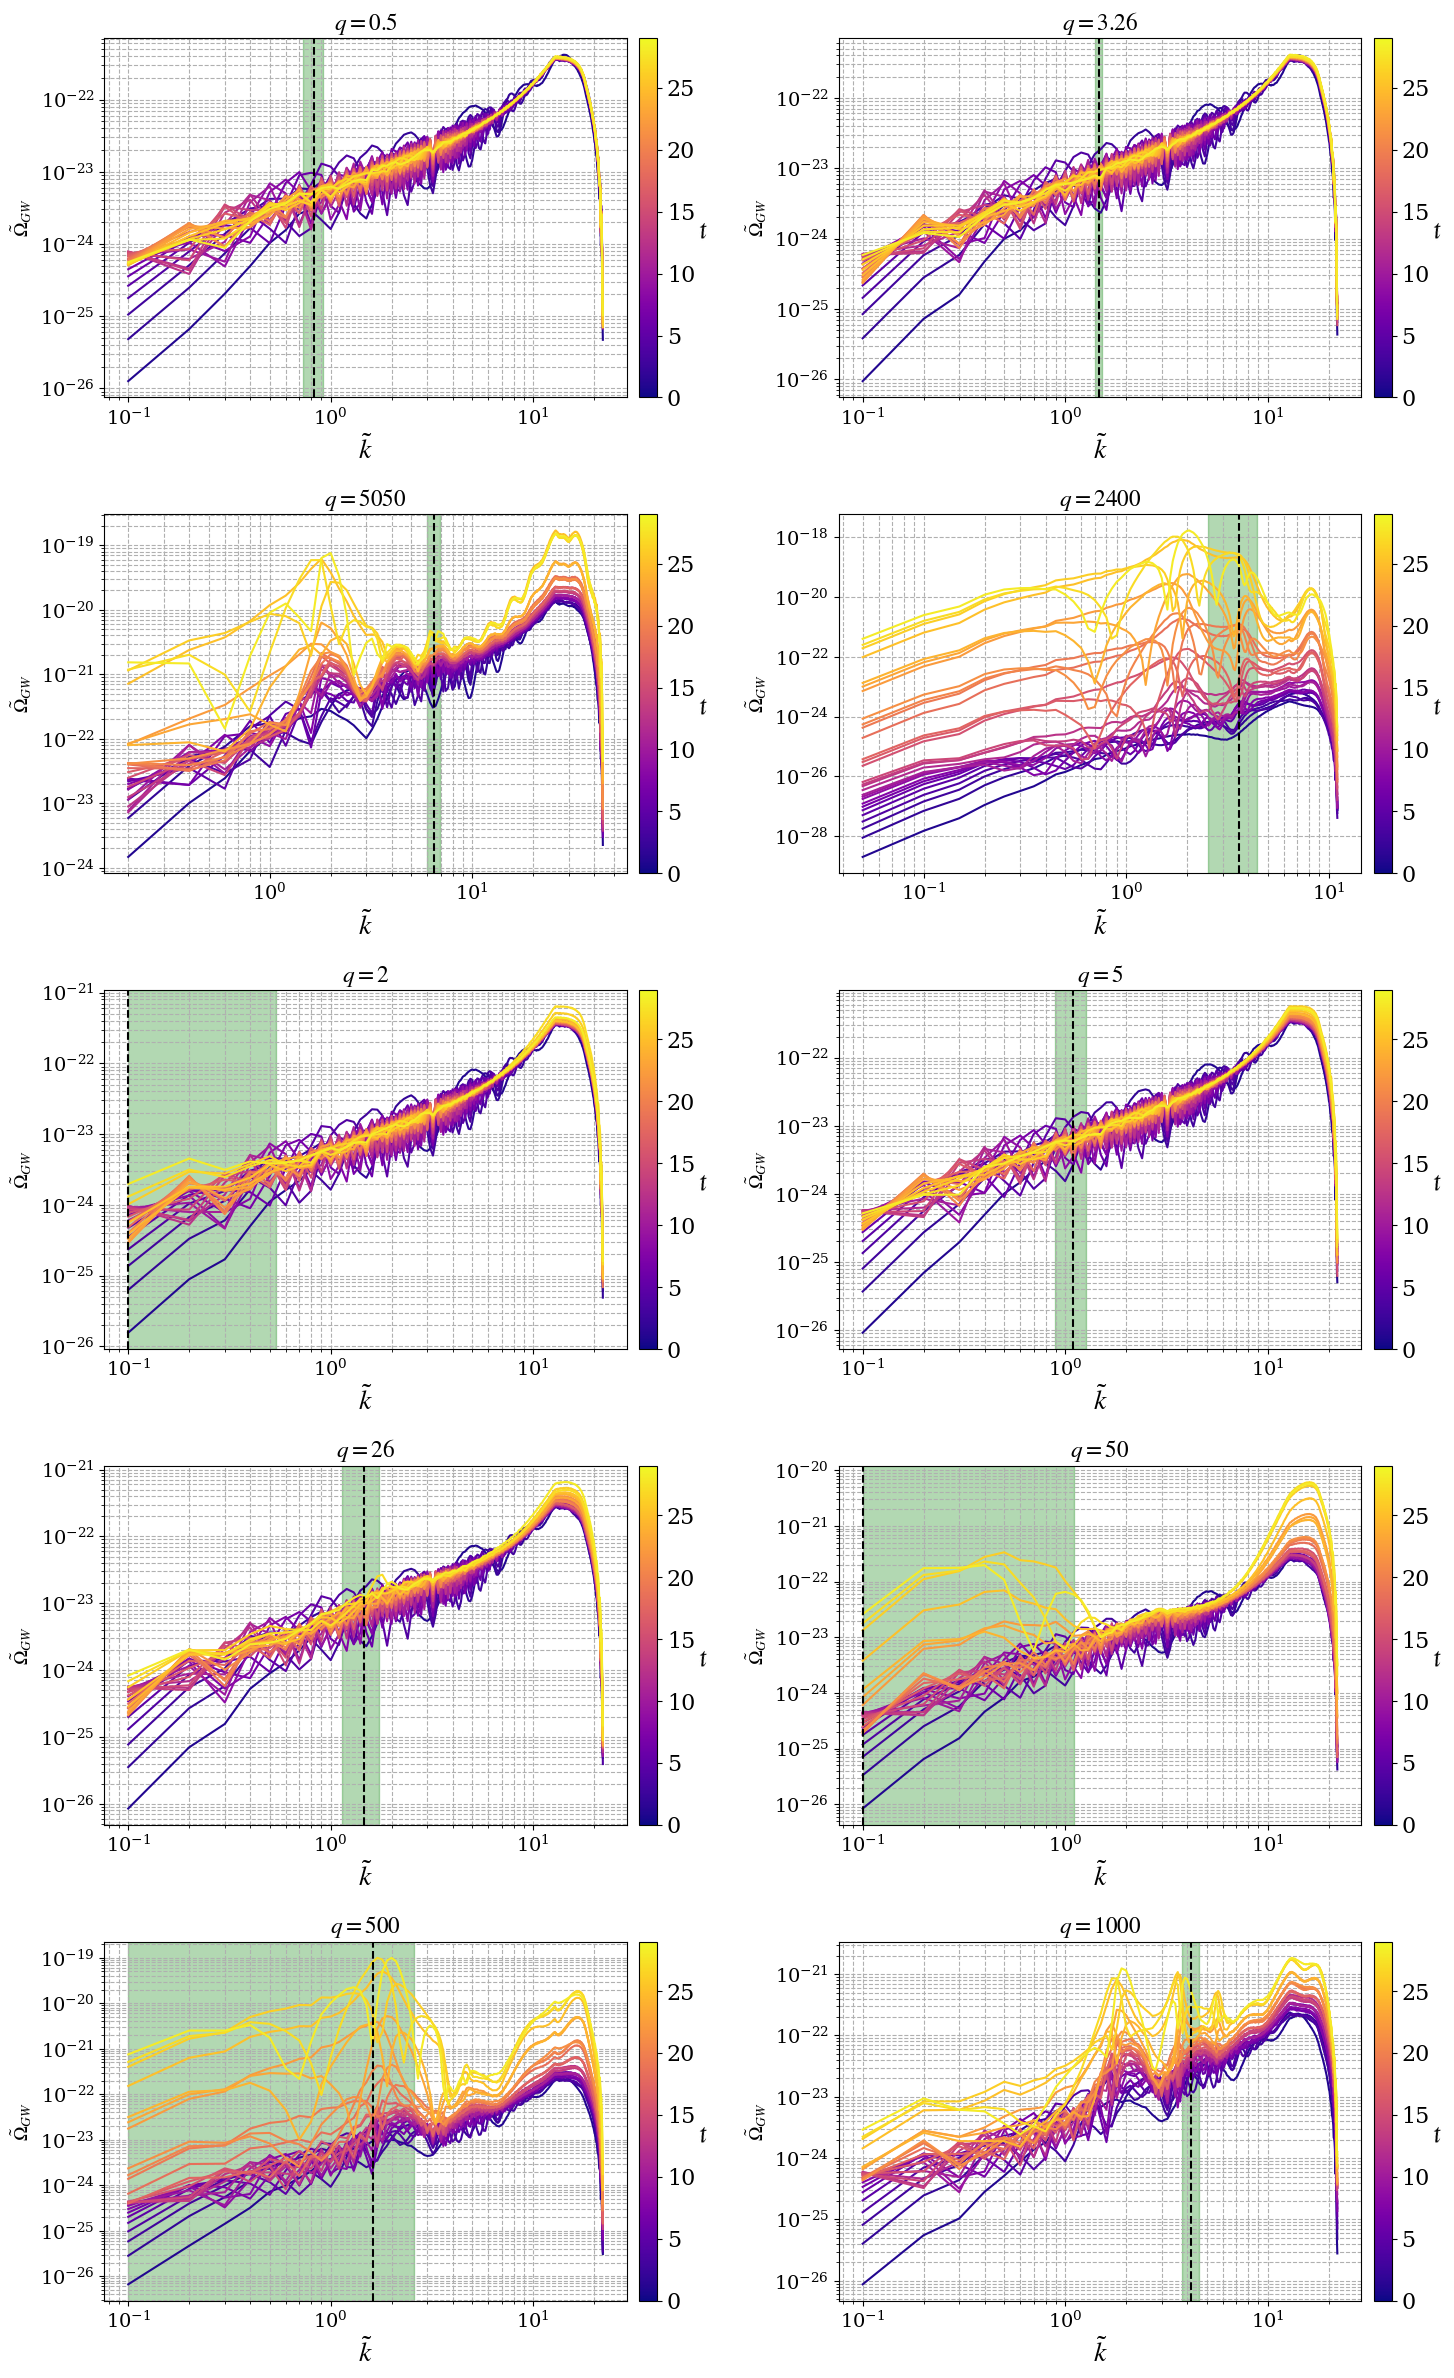
\includegraphics[width = \linewidth]{Imagenes/cosmolattice/varq_GW.png}
    \caption{espectro de ondas gravitacionales para distintos $q$.}
    \label{fig:cosmolattice_varq_GW}
\end{figure}

En estos últimos espectros podemos notar que el pico de resonancia dónde se amplifica fuertemente el espectro, tenemos que dónde ocurre una narrow resonance ($q$ chicos) el pico casi no se nota y se homogeniza rápido el espectro, mientras que cuando ocurre broad resonance ($q$ grandes) el pico se nota amplificado y coincide con la posición esperada del pico. 

\subsection{Modelo de Starobinsky}

El modelo de Starobinsky lo podemos pensar como el siguiente potencial:

\begin{equation}
    V(\phi) = \frac{3}{4} M^2 M^2_{Pl} \left[ 1 - \exp \left( - \sqrt{\frac{2}{3}} \frac{\phi}{M_{pl}} \right) \right]^2
\end{equation}

\noindent
por tanto si queremos adimensionalizar este potencial vamos a tener que definir un $\tilde{\phi} = \phi/M_{pl}$ lo que hará que el potencial nos quede:

\begin{equation}
    V(\phi) = \frac{3}{4} M^2 M^2_{Pl} \left[ 1 - \exp \left( - \sqrt{\frac{2}{3}} \tilde{\phi} \right) \right]^2
\end{equation}

\noindent
luego, nos falta adimensionalizar la amplitud del potencial para ello podemos notar que nuestra escala de energía típica es $M^2 M_{Pl}^2$ entonces podemos definir un potencial adimensional de la siguiente forma:

\begin{equation}
    \tilde{V} (\phi) = \frac{3}{4} \left[ 1 - \exp \left( - \sqrt{\frac{2}{3}} \tilde{\phi} \right) \right]^2
\end{equation}

Comparando con los archivos de CosmoLattice, ésto implica que vamos a necesitar tomar $f_* = M_{Pl}$ y $\omega_* = M$. Y con ello en mente, podemos armarnos nuestro \texttt{.h}, pero siguiendo la línea de \url{https://arxiv.org/pdf/2409.05615} vamos a definir dos parámetros $\kappa$ y $\gamma$ para variar en nuestro modelo (los llamo así para que no tenga problemas con las variables de CosmoLattice) tal que el potencial queda:

\begin{equation}
    \tilde{V} (\phi) = \kappa \left[ 1 - \exp \left( - \sqrt{\frac{2}{3 \gamma}} \tilde{\phi} \right) \right]^2
\end{equation}

\begin{infobox}[ForestGreen]{Calculos Auxiliares}
    \begin{equation*}
        \begin{split}
            \tilde{V}^\prime \left( \tilde{\phi} \right) &= 2 \kappa \left[ 1 - \exp \left( - \sqrt{\frac{2}{3 \gamma}} \tilde{\phi} \right) \right] \cdot \left[ - \sqrt{\frac{2}{3 \gamma}} \exp \left( - \frac{2}{3 \gamma} \tilde{\phi} \right) \right]\\
            \tilde{V}^\prime \left( \tilde{\phi} \right) &= - 2 \sqrt{\frac{2}{3 \gamma}} \kappa \left[ \exp \left( - \sqrt{\frac{2}{3 \gamma}} \tilde{\phi} \right) - \exp \left( - 2 \sqrt{\frac{2}{3 \gamma}} \tilde{\phi} \right) \right]
        \end{split}
    \end{equation*}

    \begin{equation*}
        \begin{split}
            V^{\prime \prime} \left( \tilde{\phi} \right) &= - 2 \sqrt{\frac{2}{3 \gamma}} \kappa \left[ - \sqrt{\frac{2}{3 \gamma}} \exp \left( - \sqrt{\frac{2}{3 \gamma}} \tilde{\phi} \right) + 2 \sqrt{\frac{2}{3 \gamma}} \exp \left( - 2 \sqrt{\frac{2}{3 \gamma}} \tilde{\phi} \right) \right]\\
            V^{\prime \prime} \left( \tilde{\phi} \right) &= \frac{4 \kappa}{3 \gamma} \left[ \exp \left( - \sqrt{\frac{2}{3 \gamma}} \tilde{\phi} \right) - 2 \exp \left( - 2 \sqrt{\frac{2}{3 \gamma}} \tilde{\phi} \right) \right] 
        \end{split}
    \end{equation*}
\end{infobox}

\noindent
con todo ésto, el \texttt{.h} queda:

\begin{lstlisting}[style = cppStyle]
#ifndef STAROBINSKY3_H //Usual macro guard to prevent multiple inclusion
#define STAROBINSKY3_H

#include "CosmoInterface/cosmointerface.h"

//Include cosmointerface to have access to all of the library.

namespace TempLat
{
    /////////
    // Model name and number of fields
    /////////

    // In the following class, we define the defining parameters of your model:
    //number of fields of each species and the type of interactions.

    struct ModelPars : public TempLat::DefaultModelPars {
        static constexpr size_t NScalars = 2;
        static constexpr size_t NPotTerms = 2;
        // Our potential naturaly splits into two terms: the inflaton potential
        // and the interaction with the daughter field.
    };

  #define MODELNAME starobinsky3
  // Here we define the name of the model. This should match the name of your file.

  template<class R>
  using Model = MakeModel(R, ModelPars);

  class MODELNAME : public Model<MODELNAME>
  //Declaration of our model. It inherits from the generic model defined above.
  {
 //...
private:

	double M, Lambda4, phii, omega, q, g;

// fldS0, piS0 : arrays which should contain the initial homogeneous values of
//               the scalar fields
//
// alpha, fStar, omegaStar : time and field rescaling to go to program units.
//
// fldS : The actual object which contains the scalar fields.
  
  public:

    MODELNAME(ParameterParser& parser, RunParameters<double>& runPar, std::shared_ptr<MemoryToolBox> toolBox): //Constructor of our model.
    Model<MODELNAME>(parser,runPar.getLatParams(), toolBox, runPar.dt, STRINGIFY(MODELLABEL)) //MODELLABEL is defined in the cmake.
    {
      /////////
      // Independent parameters of the model and initial homogeneous components of the fields
      /////////
      
        M = parser.get<double>("M");
        Lambda4 = parser.get<double>("Lambda4");
        q = parser.get<double>("q");
        
        fldS0 = parser.get<double, 2>("initial_amplitudes");
        piS0 = parser.get<double, 2>("initial_momenta", {0, 0});
        
        phii = fldS0[0];
        g = sqrt(q)*omega/phii;
        omega = sqrt(Lambda4  / pow<2>(M)); 

        
        /////////
        // Rescaling for program variables
        /////////
        
    alpha = 0; //0 coordinate time, 1 conformal time
   	fStar = fldS0[0];
   	omegaStar = omega;
   		 

   		 setInitialPotentialAndMassesFromPotential();
   		
   	}
   		 
   /////////
   // Program potential (add as many functions as terms are in the potential)
   /////////  
   
    auto potentialTerms(Tag<0>) // Inflaton potential energy
    {
      	return pow<2>(M/phii) * pow<2>(1-exp(-fldS(0_c)*phii/M)) / 2;
    }
    auto potentialTerms(Tag<1>) // Interaction energy
    {
        return 0.5 * q * fldS(0_c) * fldS(0_c) * fldS(1_c) * fldS(1_c);
    }
    
    
   /////////
   // Derivatives of the program potential with respect fields (add one function for each field)
   ///////// 

    auto potDeriv(Tag<0> f0) // Derivative with respect inflaton
    {
        return   (M/phii) * (1-exp(-fldS(0_c)*phii/M)) * exp(-fldS(0_c)*phii/M)  + q * fldS(0_c) * fldS(1_c) * fldS(1_c);
    }

    auto potDeriv(Tag<1> f1)  // Derivative with respect daughter field
    {
        return  q * fldS(1_c) * fldS(0_c) * fldS(0_c);
    }
    
   /////////
   //  Second derivatives of the program potential with respect fields (add one function for each field)
   /////////

    auto potDeriv2(Tag<0> f0) // Second derivative with respect inflaton
    {
        return  ( 2 - exp( fldS(0_c) * phii / M ) ) * exp(- 2 * fldS(0_c) * phii / M ) +  q * fldS(1_c) * fldS(1_c) ;
    }

    auto potDeriv2(Tag<1> f1) // Second derivative with respect daughter field
    {
        return  q * fldS(0_c) * fldS(0_c) ;
    }

    };
}

#endif //STAROBINSKY3_H
\end{lstlisting}

Calculemos las condiciones iniciales para este potencial, para ello, veamos que la condición inicial del campo estará dada por pedir que el parámetro $\epsilon$ de slow-roll valga 1

\begin{equation*}
    \begin{split}
        \epsilon &= 1\\
        \frac{M_p^2}{2} \left[ \frac{\partial_\phi V(\phi_0)}{V(\phi_0)} \right]^2 &= 1\\
        \frac{M_p^2}{2} \left[ \frac{\partial_{\phi} \tilde{\phi} \cdot \partial_{\tilde{\phi}} V(\tilde{\phi}_0)}{V(\tilde{\phi}_0)} \right]^2 &= 1\\
        \frac{\colorcancel{red}{M_p^2}}{2} \left\{ \frac{1}{\colorcancel{red}{M_p}} \cdot \frac{- 2 \sqrt{\frac{2}{3 \gamma}} \colorcancel{ForestGreen}{\kappa} \left[ \exp \left( - \sqrt{\frac{2}{3 \gamma}} \tilde{\phi}_0 \right) - \exp \left( - 2 \sqrt{\frac{2}{3 \gamma}} \tilde{\phi}_0 \right) \right]}{\colorcancel{ForestGreen}{\kappa} \left[ 1 - \exp \left( - \sqrt{\frac{2}{3 \gamma}} \tilde{\phi}_0 \right) \right]^2} \right\}^2 &= 1\\
        \left\{ \frac{- 2 \sqrt{\frac{2}{3 \gamma}} \colorcancel{violet}{\left[ 1 - \exp \left( - \sqrt{\frac{2}{3 \gamma}} \tilde{\phi}_0 \right) \right]} \cdot \exp \left( - \sqrt{\frac{2}{3 \gamma}} \tilde{\phi}_0 \right)}{\left[ 1 - \exp \left( - \sqrt{\frac{2}{3 \gamma}} \tilde{\phi}_0 \right) \right]^{\colorcancel{violet}{2}}} \right\}^2 &= 2\\
        \frac{4}{3 \gamma} \left[ \frac{\colorcancel{blue}{\exp \left( - \sqrt{\frac{2}{3 \gamma}} \tilde{\phi}_0 \right)}}{\colorcancel{blue}{\exp \left( - \sqrt{\frac{2}{3 \gamma}} \tilde{\phi}_0 \right)} \left[ \exp \left( \sqrt{\frac{2}{3 \gamma}} \tilde{\phi}_0 \right) - 1 \right]} \right]^2 &= 2\\
        \frac{1}{\left[ \exp \left( \sqrt{\frac{2}{3 \gamma}} \tilde{\phi}_0 \right) - 1 \right]^2} &= \frac{3}{2} \gamma\\
        \exp \left( \sqrt{\frac{2}{3 \gamma}} \tilde{\phi}_0 \right) - 1 &= \sqrt{\frac{2}{3 \gamma}}\\
        \exp \left( \sqrt{\frac{2}{3 \gamma}} \tilde{\phi}_0 \right) &= \sqrt{\frac{2}{3 \gamma}} + 1\\
        \sqrt{\frac{2}{3 \gamma}} \tilde{\phi}_0 &= \ln \left( \sqrt{\frac{2}{3 \gamma}} + 1 \right)
    \end{split}
\end{equation*}

\begin{equation}
    \tilde{\phi}_0 = \sqrt{\frac{3}{2} \gamma} \ln \left( \sqrt{\frac{2}{3 \gamma}} + 1 \right)
\end{equation}

La velocidad inicial del campo inflatón la podemos plantear a partir de pedir que la energía cinética inicial sea igual a la energía potencial del campo:

\begin{equation*}
    \begin{split}
        \frac{1}{2} \dot{\tilde{\phi}}^2_0 &= V(\tilde{\phi}_0)\\
        \dot{\tilde{\phi}}_0 &= \sqrt{2 V(\tilde{\phi}_0)}\\
        \dot{\tilde{\phi}}_0 &= \sqrt{2 \kappa \left[ 1 - \exp \left( - \sqrt{\frac{2}{3 \gamma}} \tilde{\phi}_0 \right) \right]^2}\\
        \dot{\tilde{\phi}}_0 &= \sqrt{2 \kappa} \left[ 1 - \exp \left( - \sqrt{\frac{2}{3 \gamma}} \tilde{\phi}_0 \right) \right]\\ 
        \dot{\tilde{\phi}}_0 &= \sqrt{2 \kappa} \left[ 1 - \exp \left( - \sqrt{\frac{2}{3 \gamma}} \cdot \sqrt{\frac{3}{2} \gamma} \ln \left( \sqrt{\frac{2}{3 \gamma}} + 1 \right) \right) \right]\\ 
        \dot{\tilde{\phi}}_0 &= \sqrt{2 \kappa} \left[ 1 - \exp \left( - \ln \left( \sqrt{\frac{2}{3 \gamma}} + 1 \right) \right) \right]
    \end{split}
\end{equation*}

\begin{equation}
    \dot{\tilde{\phi}}_0 = \sqrt{2 \kappa} \left[ 1 - \left( \sqrt{\frac{2}{3 \gamma}} + 1 \right)^{-1} \right]
\end{equation}

Para este modelo, si utilizamos un $q = 4 \times 10^4$ podemos encontrarnos con gráficos como los que tenemos abajo, dónde de la densidad de energía (Fig. \ref{fig:densidad_Starobinsky}) se puede observar que cuando el término de los gradientes (naranja y rojo) aumentan al igual que el de la interacción tendremos producción de ondas gravitacionales, y a medida que éstos se estabilizan la producción se congela manteniendo la energía de las ondas en un valor fijo. A su vez, del espectro de potencias (Fig. \ref{fig:Omega_Starobinsky}) podemos observar que el espectro es homogéneo sin picos y por tanto sin bandas de resonancia dónde las ondas se amplifican fuertemente.

\begin{figure}[H]
    \centering
    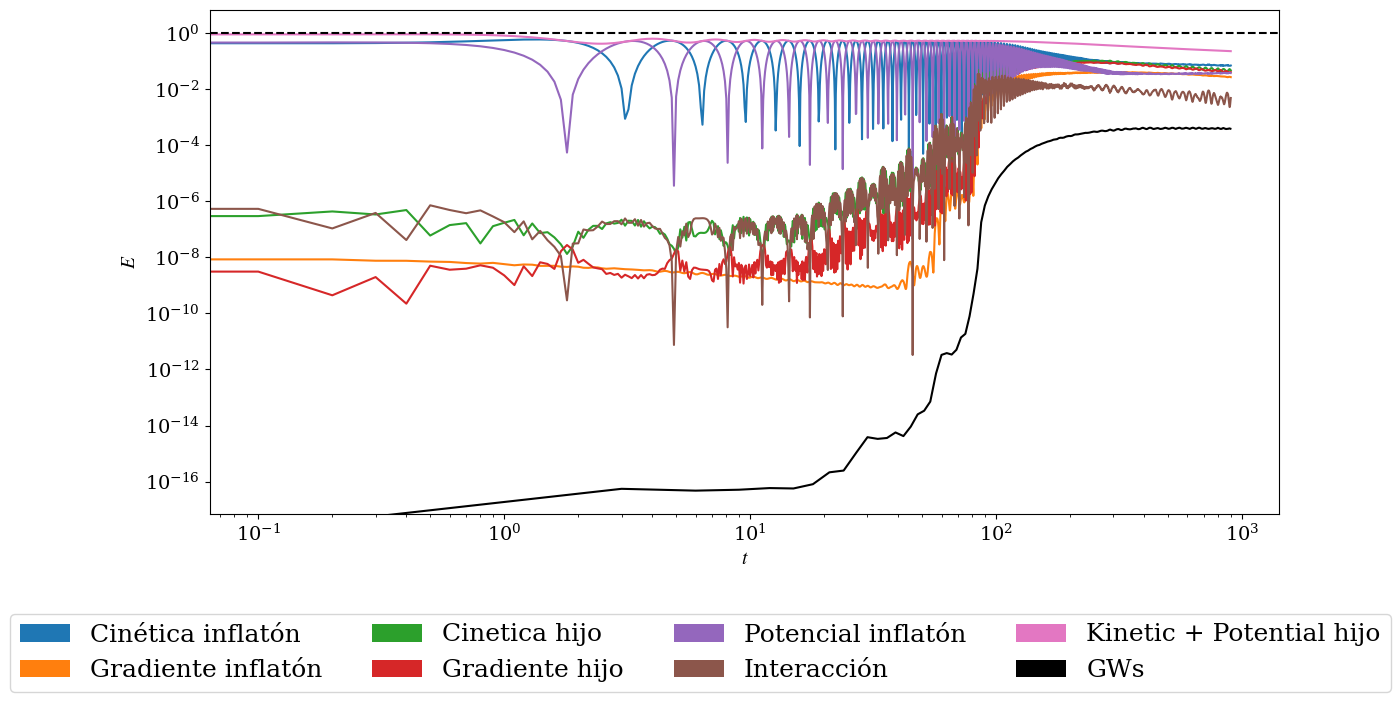
\includegraphics[width = \linewidth]{Imagenes/cosmolattice/Energia_Starobinsky.png}
    \caption{evolución en la densidad de energía de cada término de la acción y energía de las ondas gravitacionales en el tiempo en un modelo de tipo Starobinsky para $q = 4 \times 10^4$.}
    \label{fig:densidad_Starobinsky}
\end{figure}

\begin{figure}[H]
    \centering
    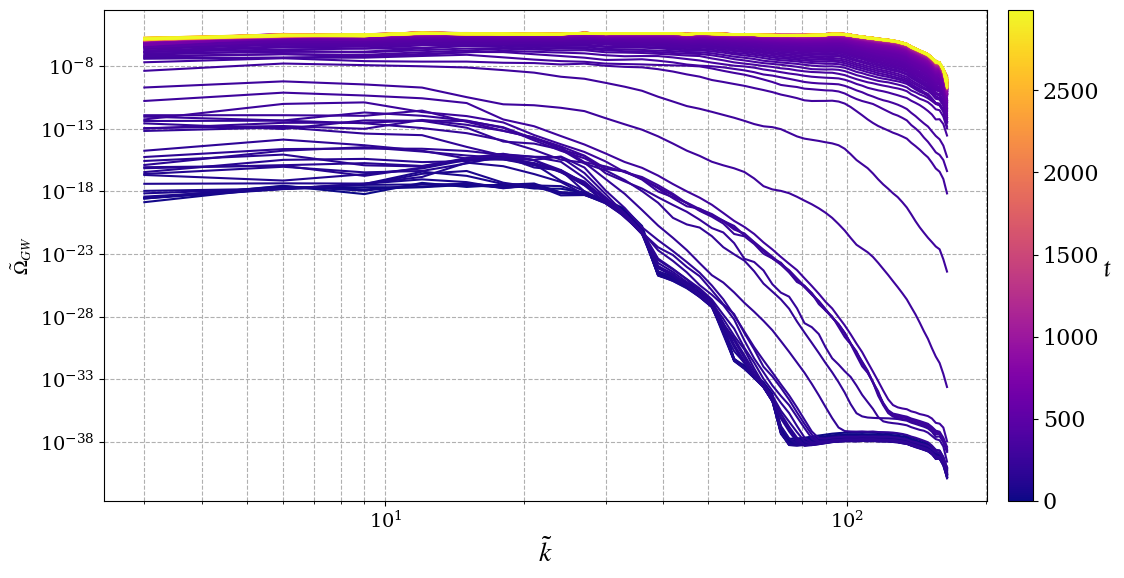
\includegraphics[width = \linewidth]{Imagenes/cosmolattice/Omega_Starobinsky.png}
    \caption{espectro de potencia para las ondas gravitacionales en un modelo de tipo Starobinsky para $q = 4 \times 10^4$.}
    \label{fig:Omega_Starobinsky}
\end{figure}

\subsection{Modelo $m^2 \phi^2$}

El modelo de $m^2 \phi^2$ tampoco se encontraba programado por defecto en CosmoLattice, por ello tuvimos que armarlo nosotros, y lo hicimos a partir del siguiente \texttt{.h}:

\begin{lstlisting}[style = cppStyle]
#ifndef M2PHI2_H
#define M2PHI2_H

#include "CosmoInterface/cosmointerface.h"

namespace TempLat
{
    struct ModelPars : public TempLat::DefaultModelPars {
        static constexpr size_t NScalars = 2;
        static constexpr size_t NPotTerms = 2;
    };

    #define MODELNAME m2phi2
  
    template<class R>
    using Model = MakeModel(R, ModelPars);
  
    class MODELNAME : public Model<MODELNAME>
    {
    private:
        double g, m, q, phii;
        
    public:
        MODELNAME(ParameterParser& parser, RunParameters<double>& runPar, std::shared_ptr<MemoryToolBox> toolBox) : 
            Model<MODELNAME>(parser, runPar.getLatParams(), toolBox, runPar.dt, STRINGIFY(MODELLABEL))
        {

            // Condiciones iniciales
            fldS0 = parser.get<double, 2>("initial_amplitudes");
            piS0 = parser.get<double, 2>("initial_momenta", {0, 0});
            phii = fldS0[0];
            
            // Parametros del modelo
            m = parser.get<double>("m");
            q = parser.get<double>("q");
            g = sqrt(q) * m / phii;
            
            // Rescaling para variables del programa
            alpha = 0; //1;
            fStar = phii;
            omegaStar = m;

            setInitialPotentialAndMassesFromPotential();
        }

        // Terminos del potencial
        auto potentialTerms(Tag<0>) // Potencial del inflaton
        {
            return 0.5 * pow<2>(fldS(0_c));
        }
        
        auto potentialTerms(Tag<1>) // Termino de interaccion
        {
            return 0.5 * q * pow<2>(fldS(0_c) * fldS(1_c));
        }

        // Derivadas del potencial
        auto potDeriv(Tag<0>) // Respecto al inflaton phi
        {
            return fldS(0_c) + q * fldS(0_c) * pow<2>(fldS(1_c));
        }

        auto potDeriv(Tag<1>) // Respecto al campo hijo chi
        {
            return q * fldS(1_c) * pow<2>(fldS(0_c));
        }

        // Derivadas segundas del potencial
        auto potDeriv2(Tag<0>) // Respecto a phi dos veces
        {
            return 1.0 + q * pow<2>(fldS(1_c));
        }

        auto potDeriv2(Tag<1>) // Respecto a chi dos veces
        {
            return q * pow<2>(fldS(0_c));
        }
    };
}

#endif // M2PHI2_H
\end{lstlisting}

Para este modelo, me encontré que es muy sensible a los cambios en los parámetros, haciendo que para valores de $q$ muy bajos la producción de ondas es casi nula y para valores de $q$ muy grandes el código colapsa rápidamente tienendo por respuesta un archivo lleno de \textit{nan} (Not a Number). Para resolver un poco el problema del colapso y comparar con el código de $\tanh^2$ y Statobinsky en las próximas subsecciones, trabajamos en tiempo coordenado\footnote{Según lo que leí el tiempo conforme para potenciales con masa tiene problemas el integrador y colapsa rápidamente, debo investigar más al respecto.}. Con todo ésto en mente, y para buscar qué valores de $q$ se le puede dar al código realizo un barrido en este parámetro y se pueden ver los datos más significativos en las figuras de abajo (para valores más grandes de $q$ el código colapsa en la 2da o 3era iteración).

\begin{figure}[H]
    \centering
    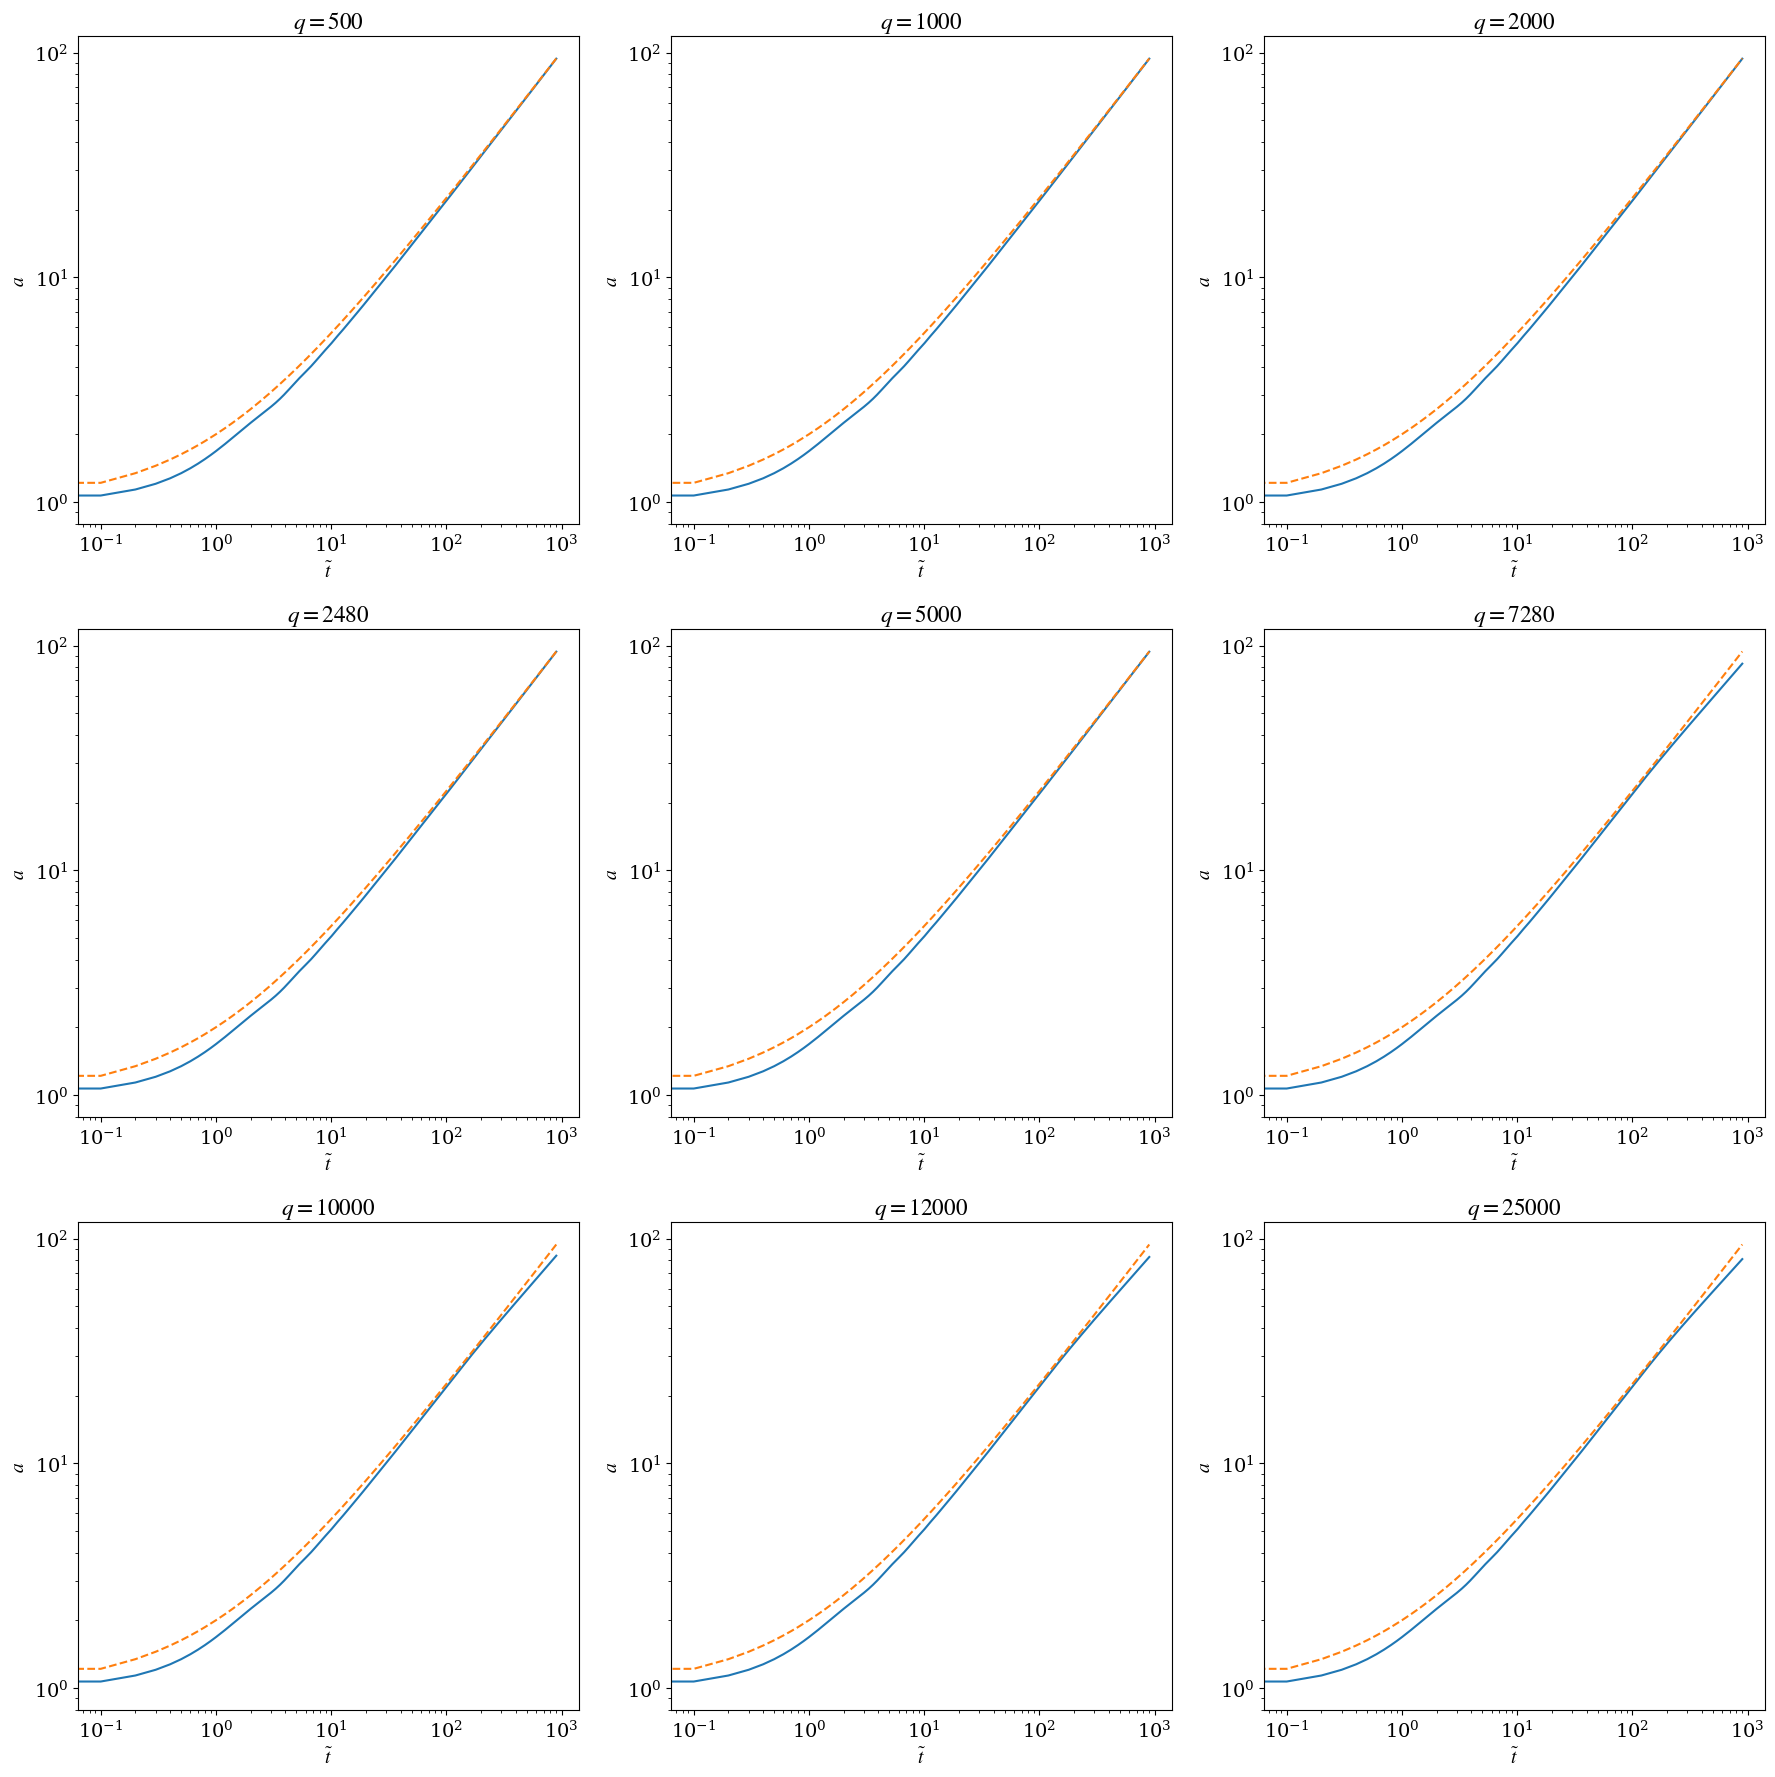
\includegraphics[width = \linewidth]{Imagenes/cosmolattice/time_evol_m2phi2.png}
    \caption{evolución de $a(t)$ para el potencial $m^2 \phi^2$, podemos ver que $a \sim t^{2/3}$.}
\end{figure}

\begin{figure}[H]
    \centering
    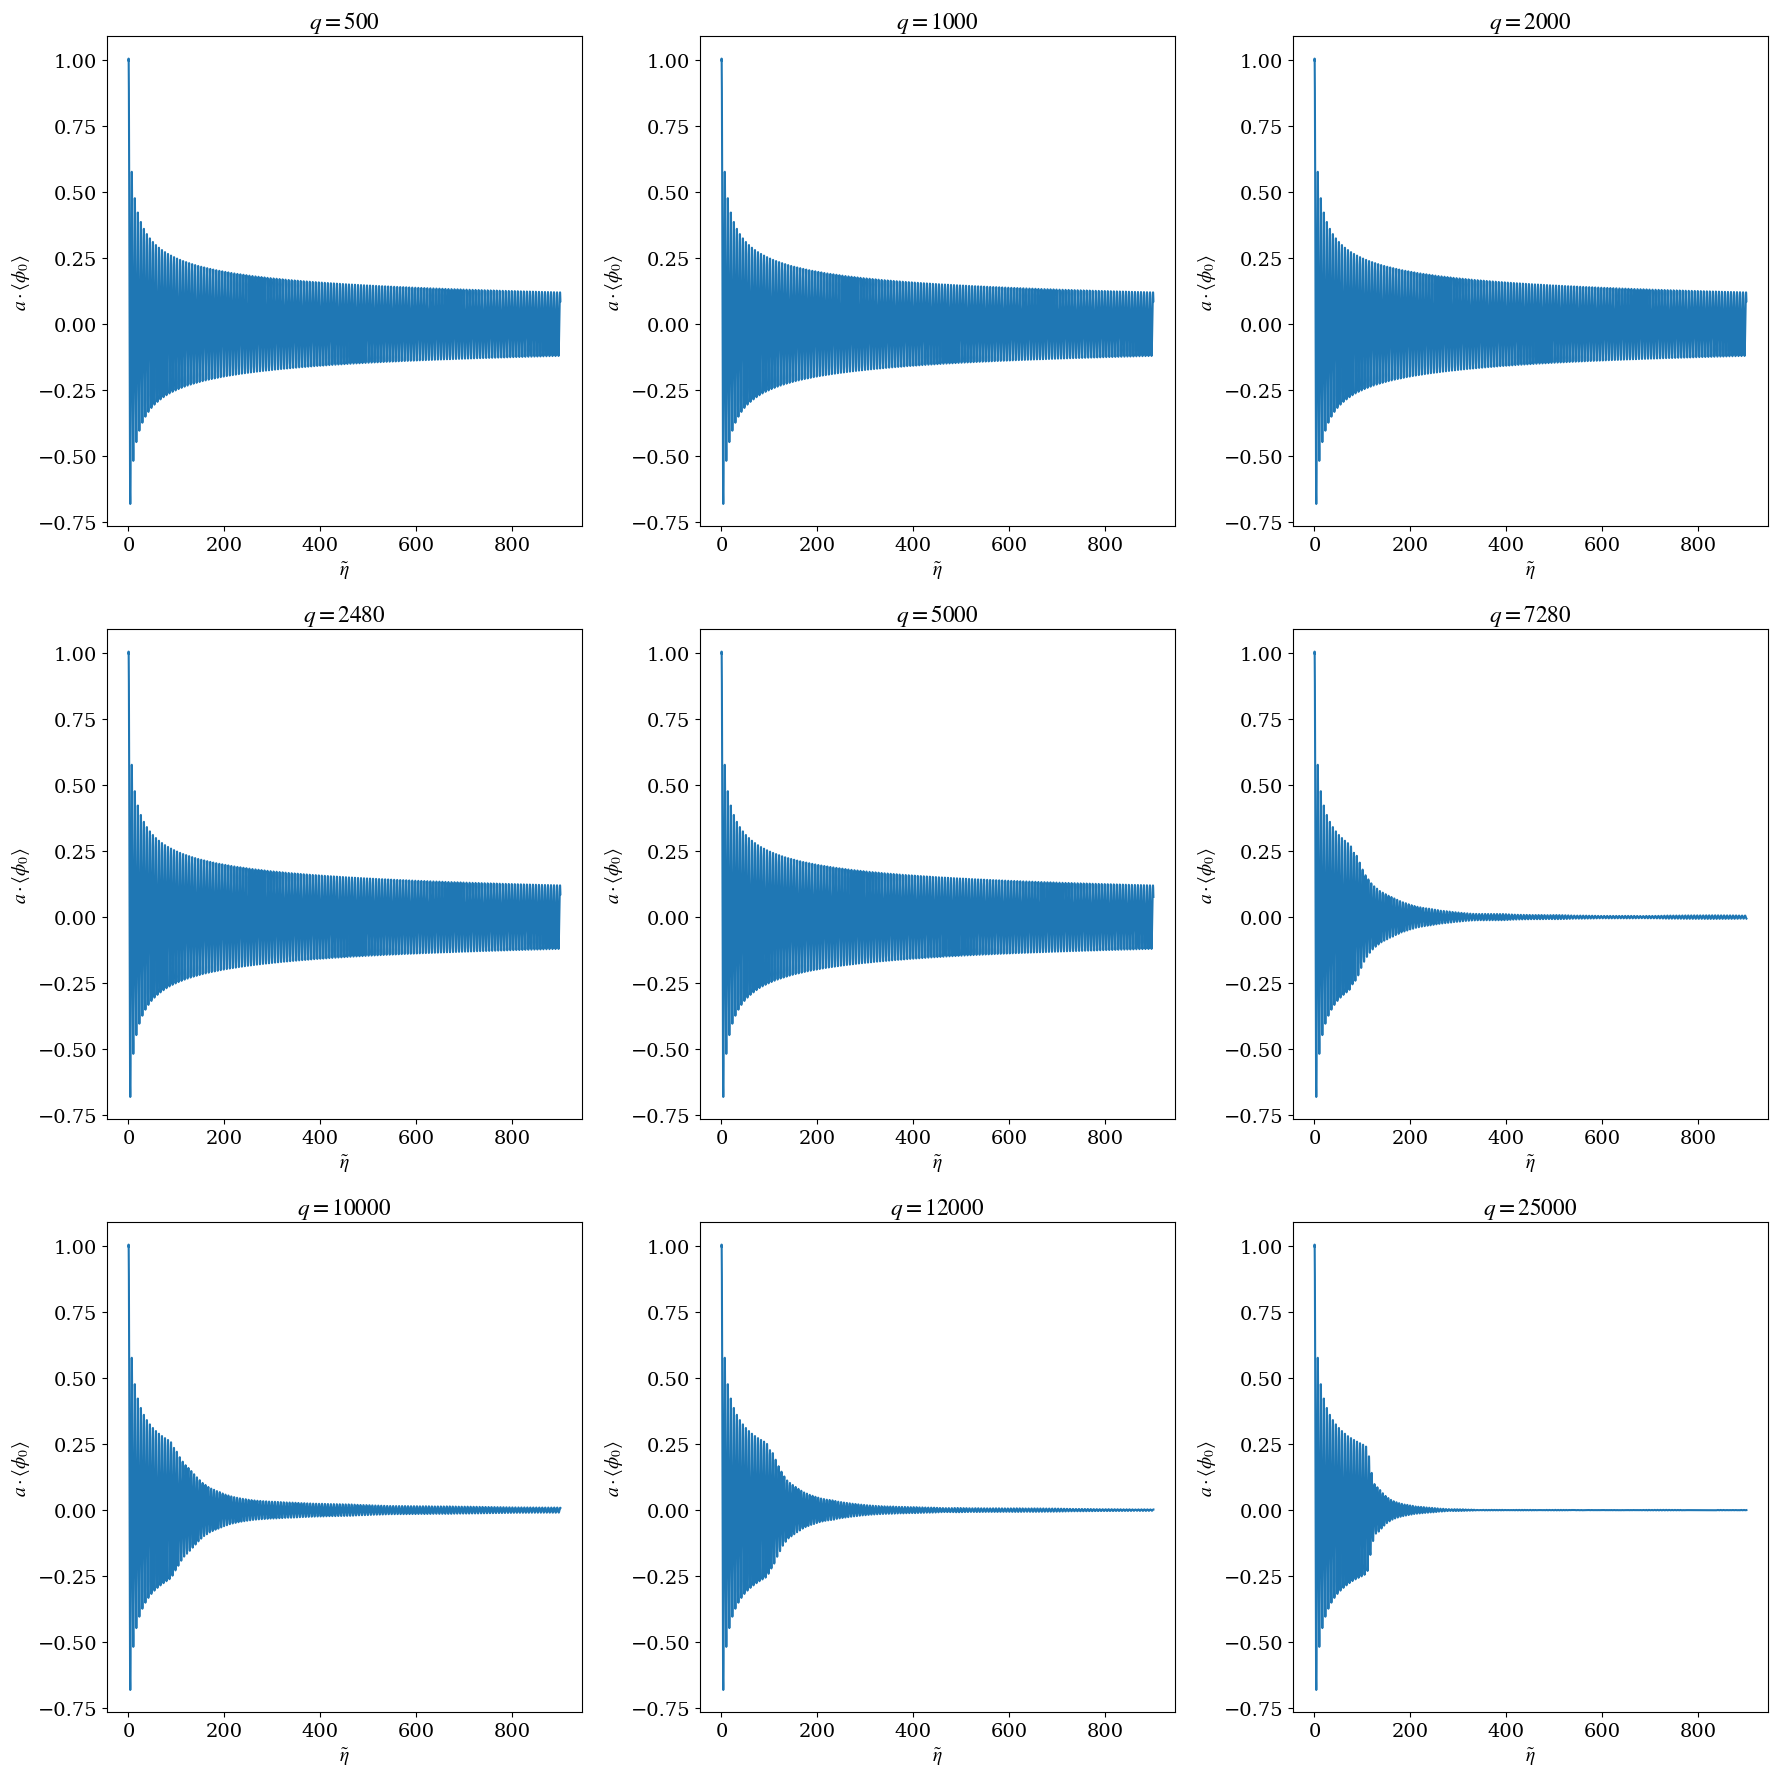
\includegraphics[width = \linewidth]{Imagenes/cosmolattice/phi_evol_m2phi2.png}
    \caption{evolución de $\phi(t)$ para el modelo $m^2 \phi^2$.}
\end{figure}

\begin{figure}[H]
    \centering
    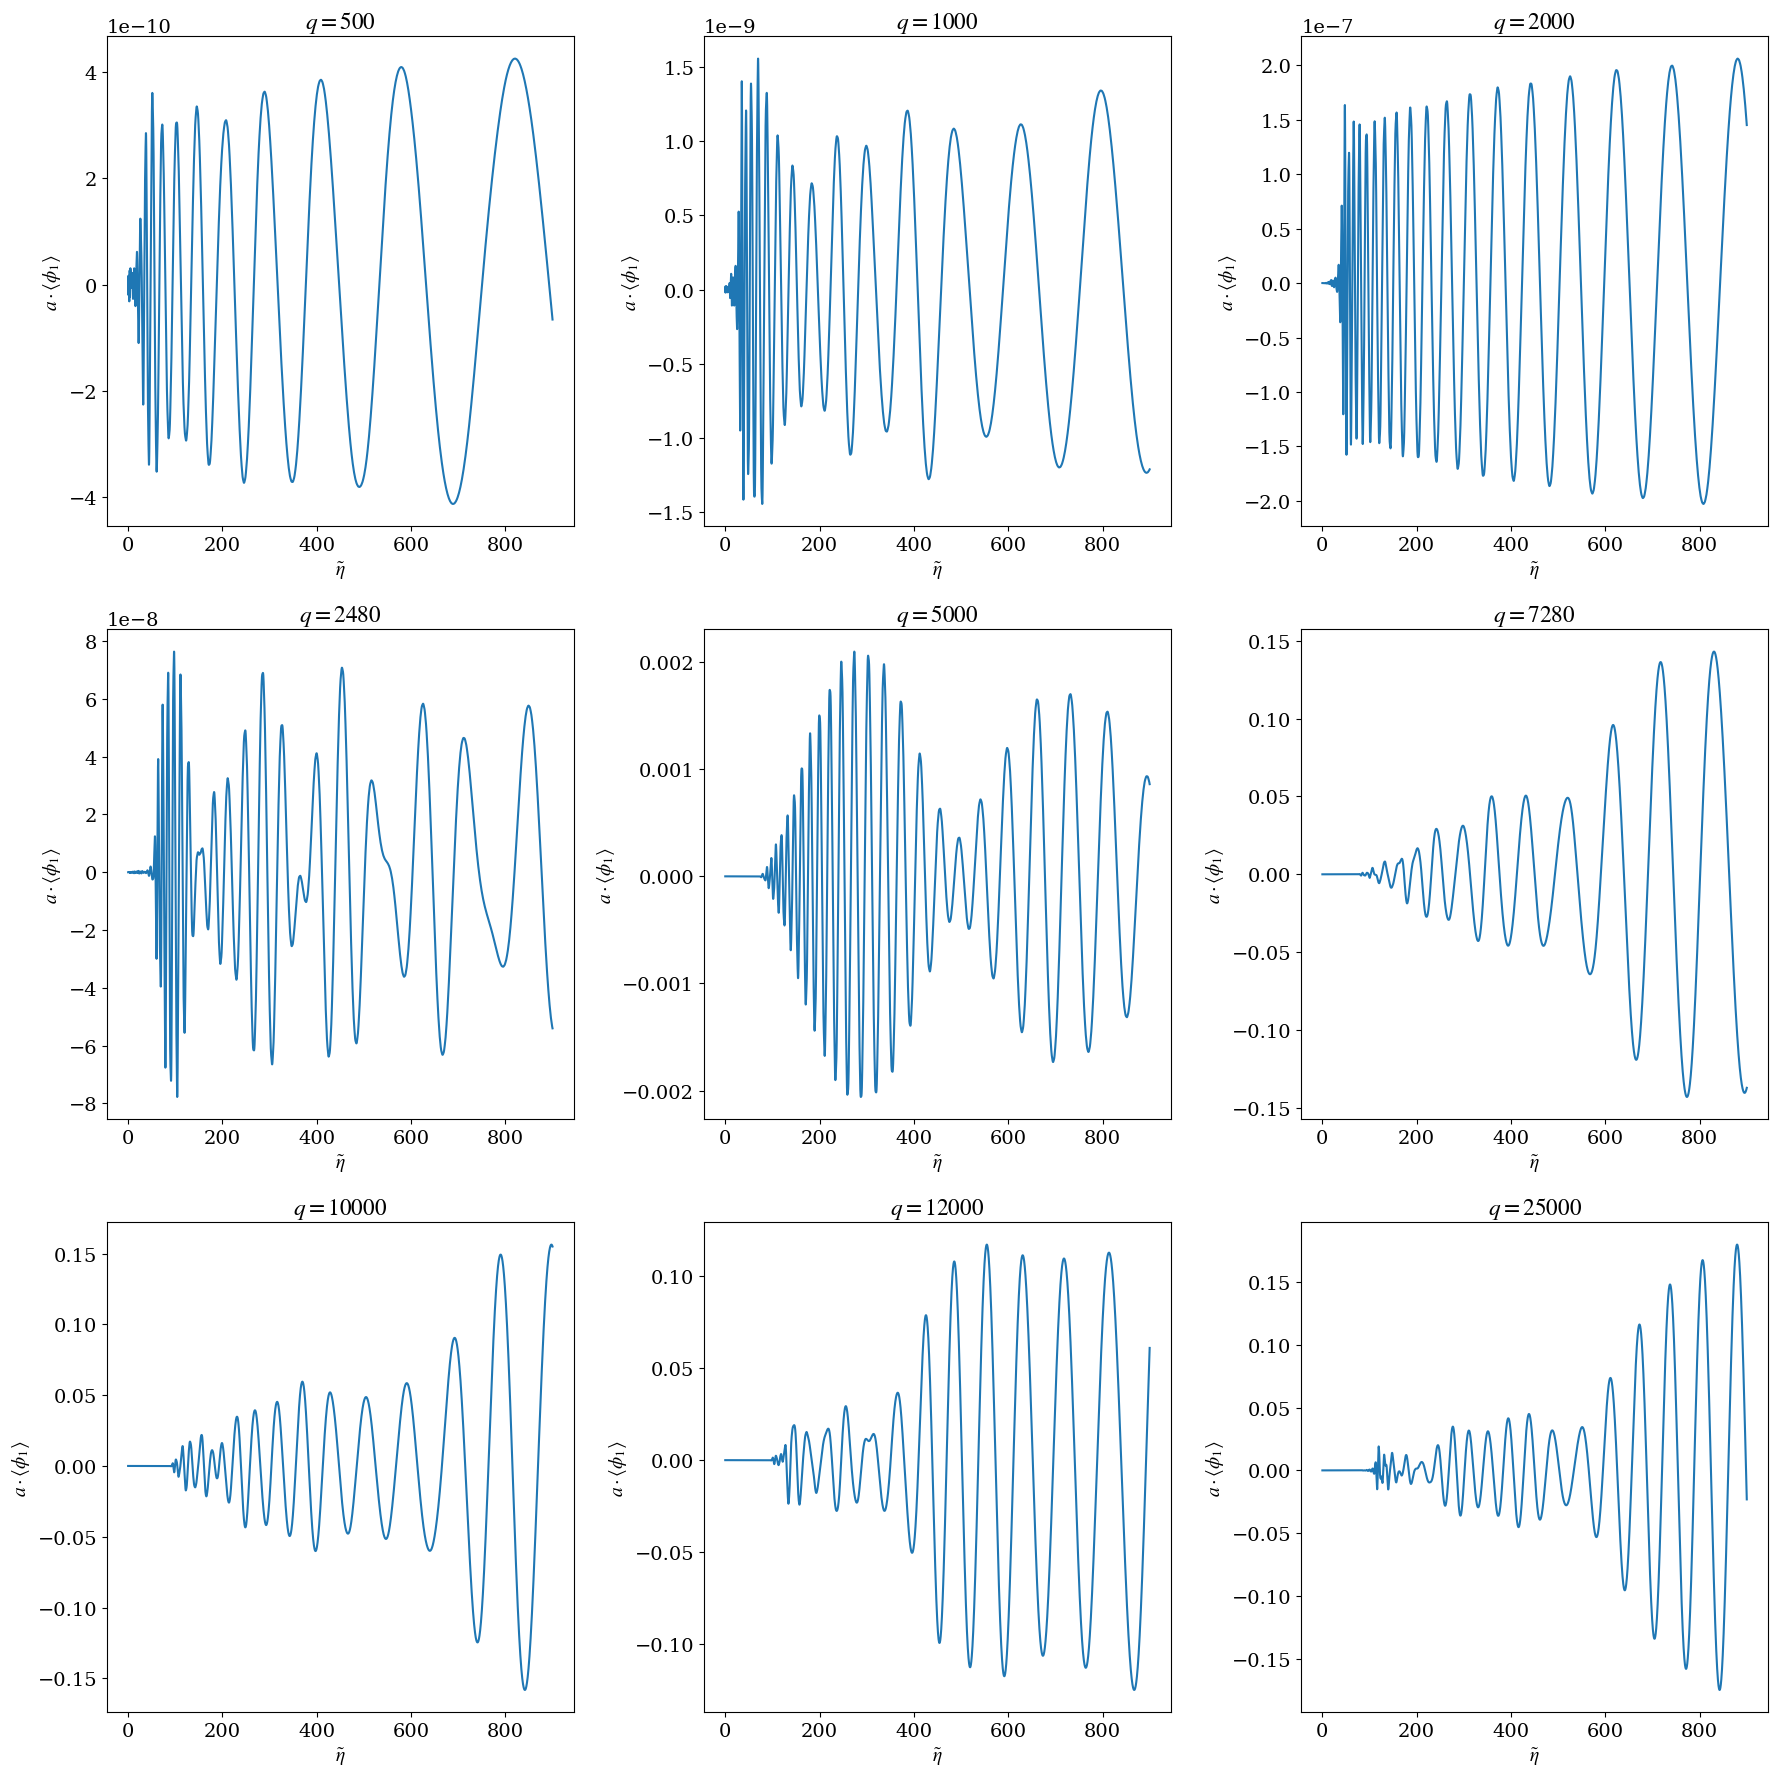
\includegraphics[width = \linewidth]{Imagenes/cosmolattice/chi_evol_m2phi2.png}
    \caption{evolución de $\chi(t)$ para el modelo $m^2 \phi^2$.}
\end{figure}

\begin{figure}[H]
    \centering
    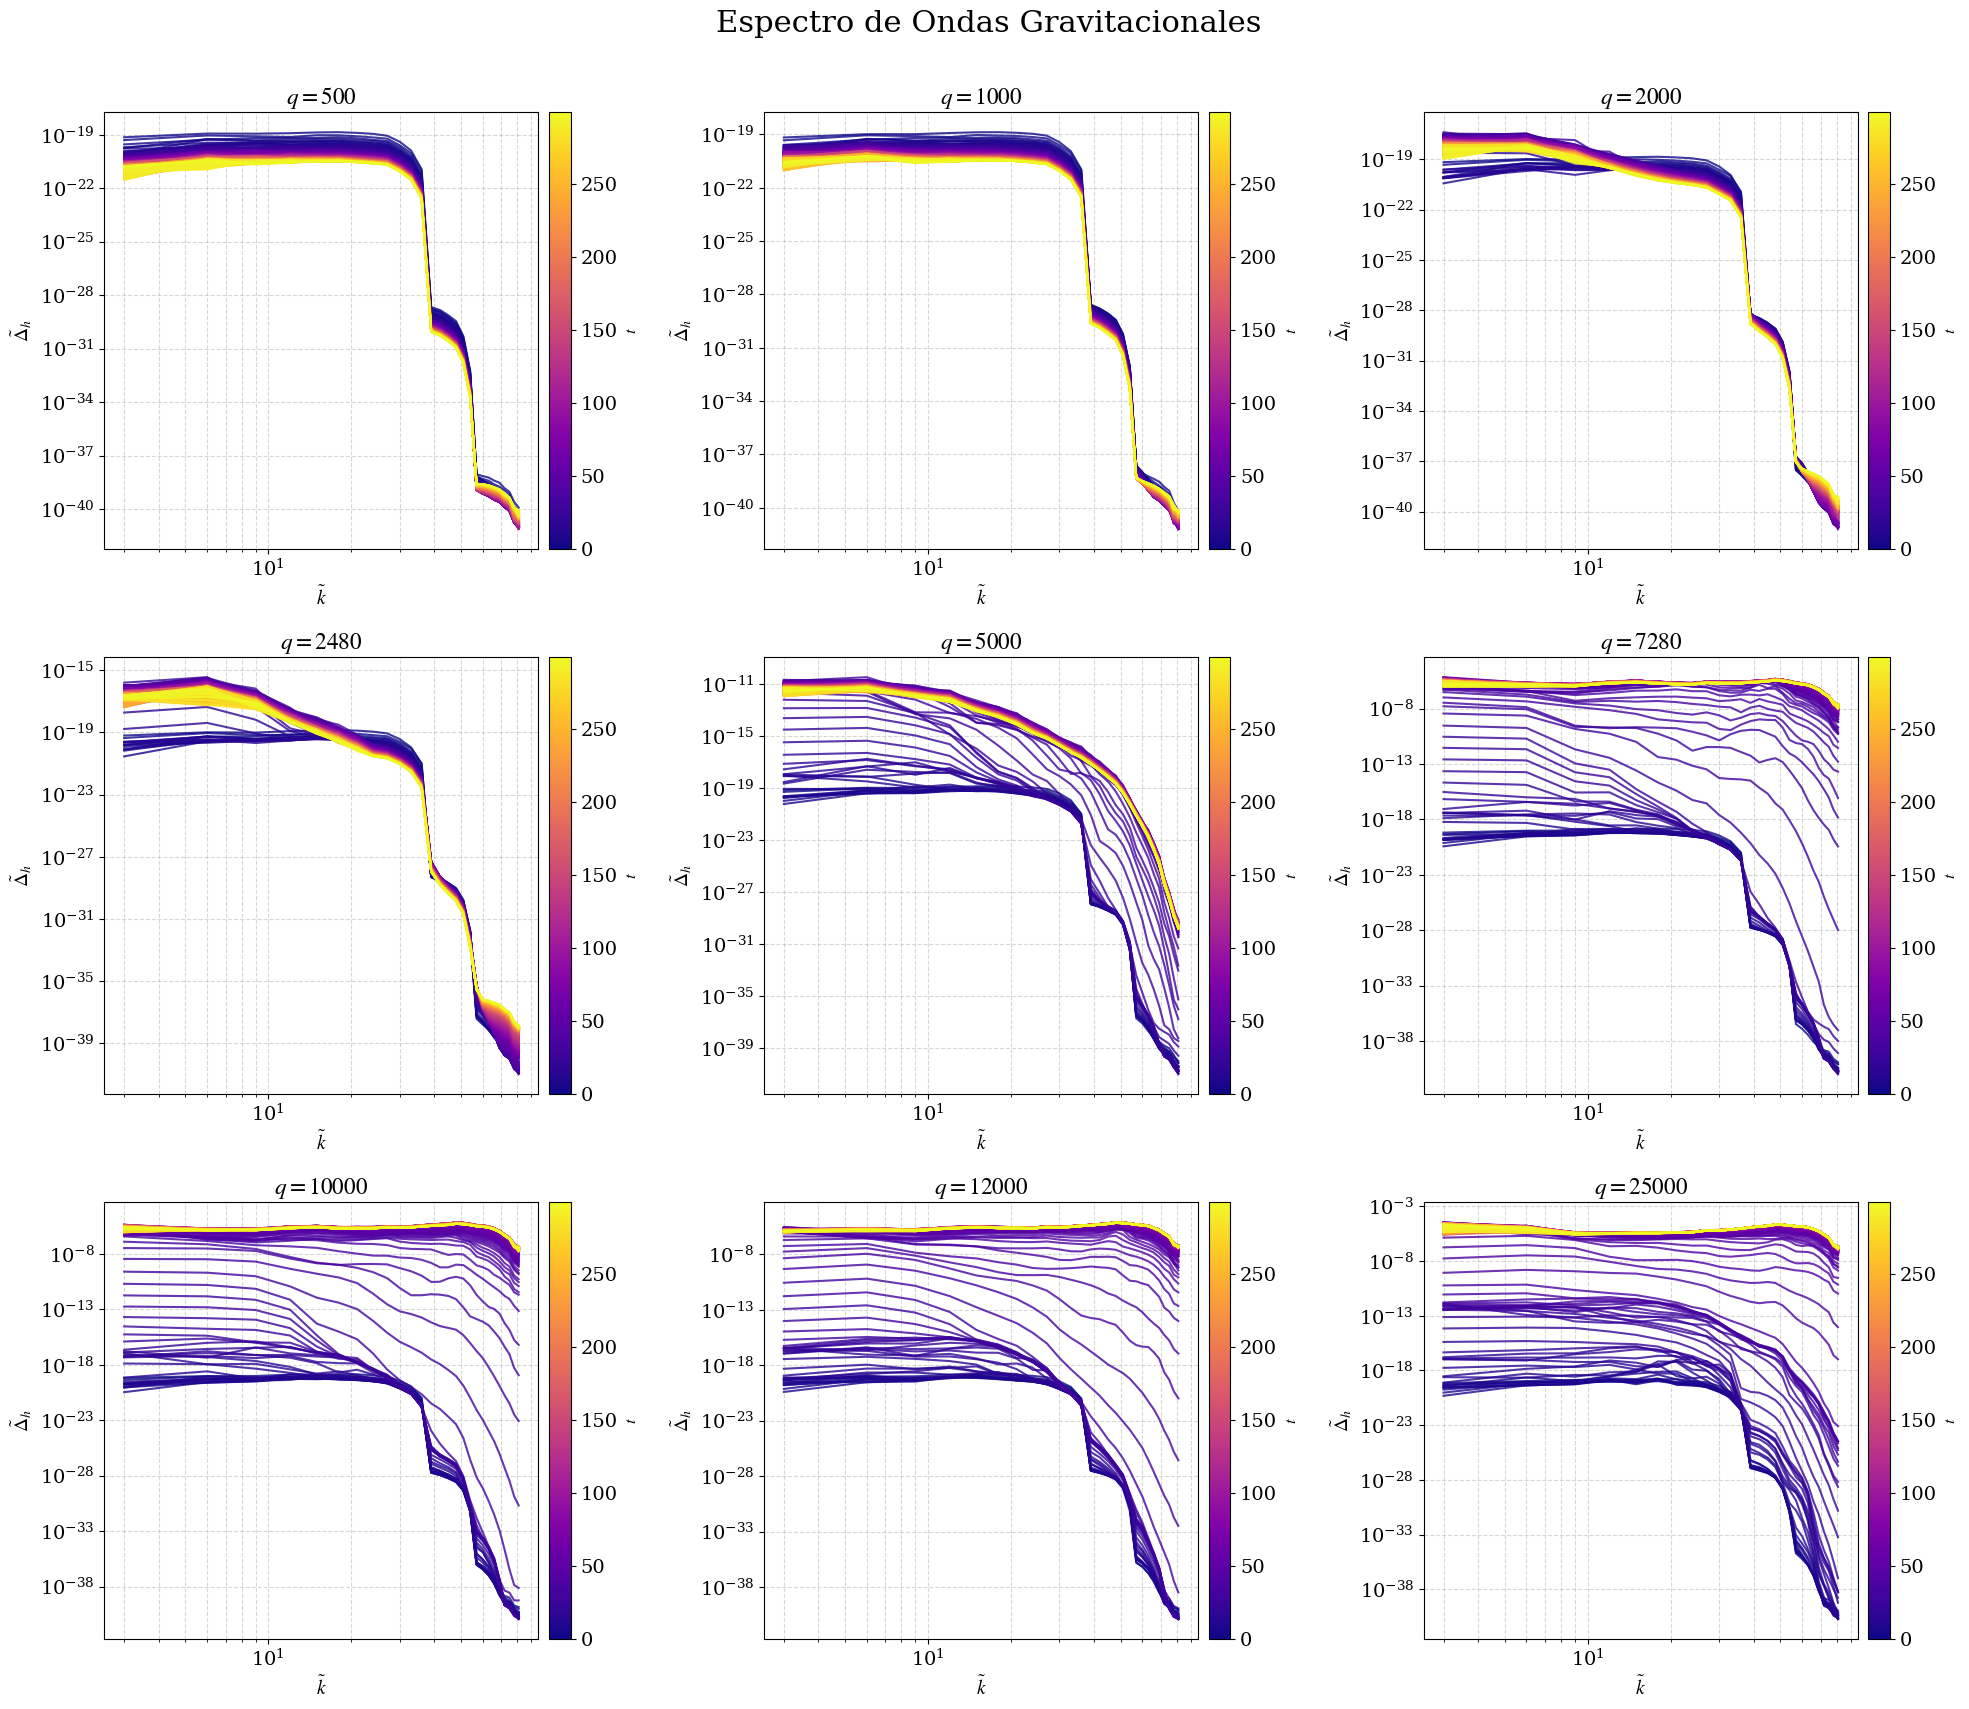
\includegraphics[width = \linewidth]{Imagenes/cosmolattice/Omega_m2phi2.png}
    \caption{espectro de potencia para las ondas gravitacionales en un modelo de tipo $m^2 \phi^2$.}
\end{figure}

\begin{figure}[H]
    \centering
    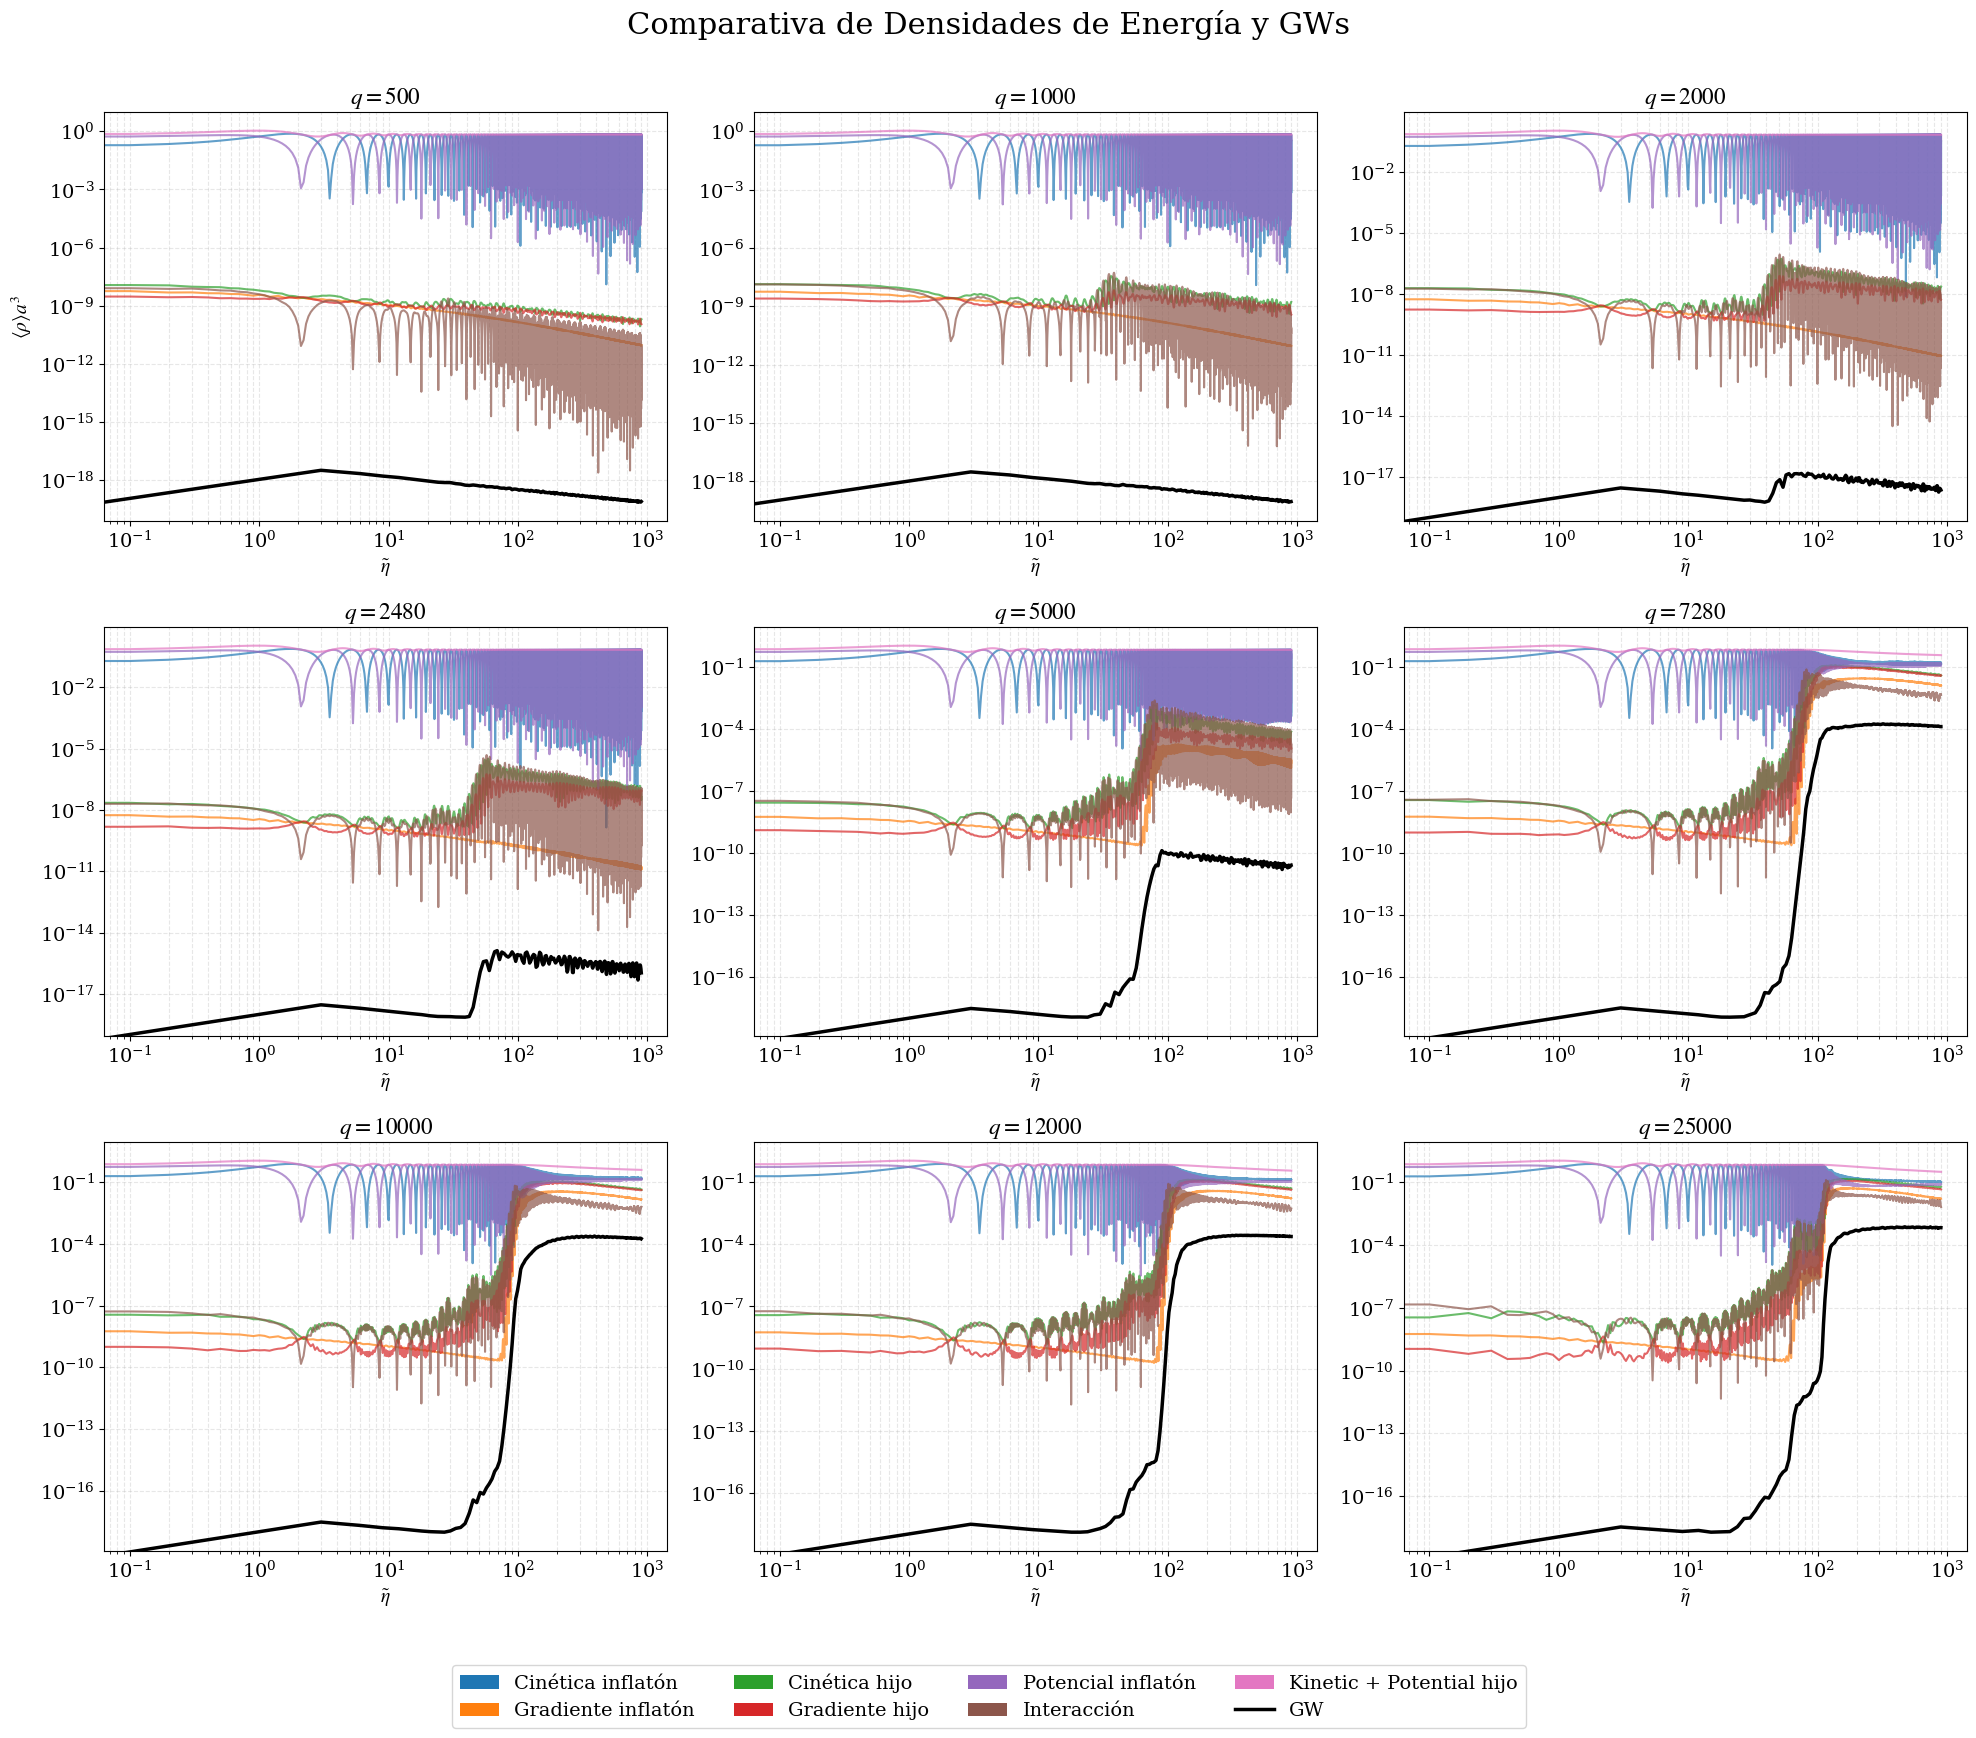
\includegraphics[width = \linewidth]{Imagenes/cosmolattice/Energy_m2phi2.png}
    \caption{evolución de las densidades de energía de cada tipo y ondas gravitacionales.}
\end{figure}

\subsection{Comparación de modelo $\lambda \phi^4$ vs. $\tanh^4$}



\subsection{Comparación de modelo $m^2 \phi^2$ vs. $\tanh^2$ vs. Starobinsky}